\documentclass[11pt,a4paper]{article}
\usepackage[utf8]{inputenc}
\usepackage{amsmath}
\usepackage{mathtools}
\usepackage{amsfonts}
\usepackage{amssymb}
\usepackage{graphicx}
\usepackage{caption}
\usepackage{subcaption}
\usepackage{comment}
\usepackage{color}
\usepackage{enumitem}
\usepackage[left=2cm,right=2cm,top=2cm,bottom=2cm]{geometry}
\usepackage{listings}
\usepackage{color}

\setlength{\jot}{10pt}
 
\definecolor{codegreen}{rgb}{0,0.6,0}
\definecolor{codegray}{rgb}{0.5,0.5,0.5}
\definecolor{codepurple}{rgb}{0.58,0,0.82}
\definecolor{backcolour}{rgb}{0.95,0.95,0.92}
 
\lstdefinestyle{mystyle}{
    backgroundcolor=\color{backcolour},   
    commentstyle=\color{codegreen},
    keywordstyle=\color{magenta},
    numberstyle=\tiny\color{codegray},
    stringstyle=\color{codepurple},
    basicstyle=\footnotesize,
    breakatwhitespace=false,         
    breaklines=true,                 
    captionpos=b,                    
    keepspaces=true,                 
    numbers=left,                    
    numbersep=5pt,                  
    showspaces=false,                
    showstringspaces=false,
    showtabs=false,                  
    tabsize=2
}
 
\lstset{style=mystyle}
\author{Andrew Teta}
\title{ECEN 4532 - Lab 2: Introduction to Image Processing}

\begin{document}

\maketitle

\begin{figure}[ht]
	\centering
	\begin{subfigure}[h]{0.6\textwidth}
		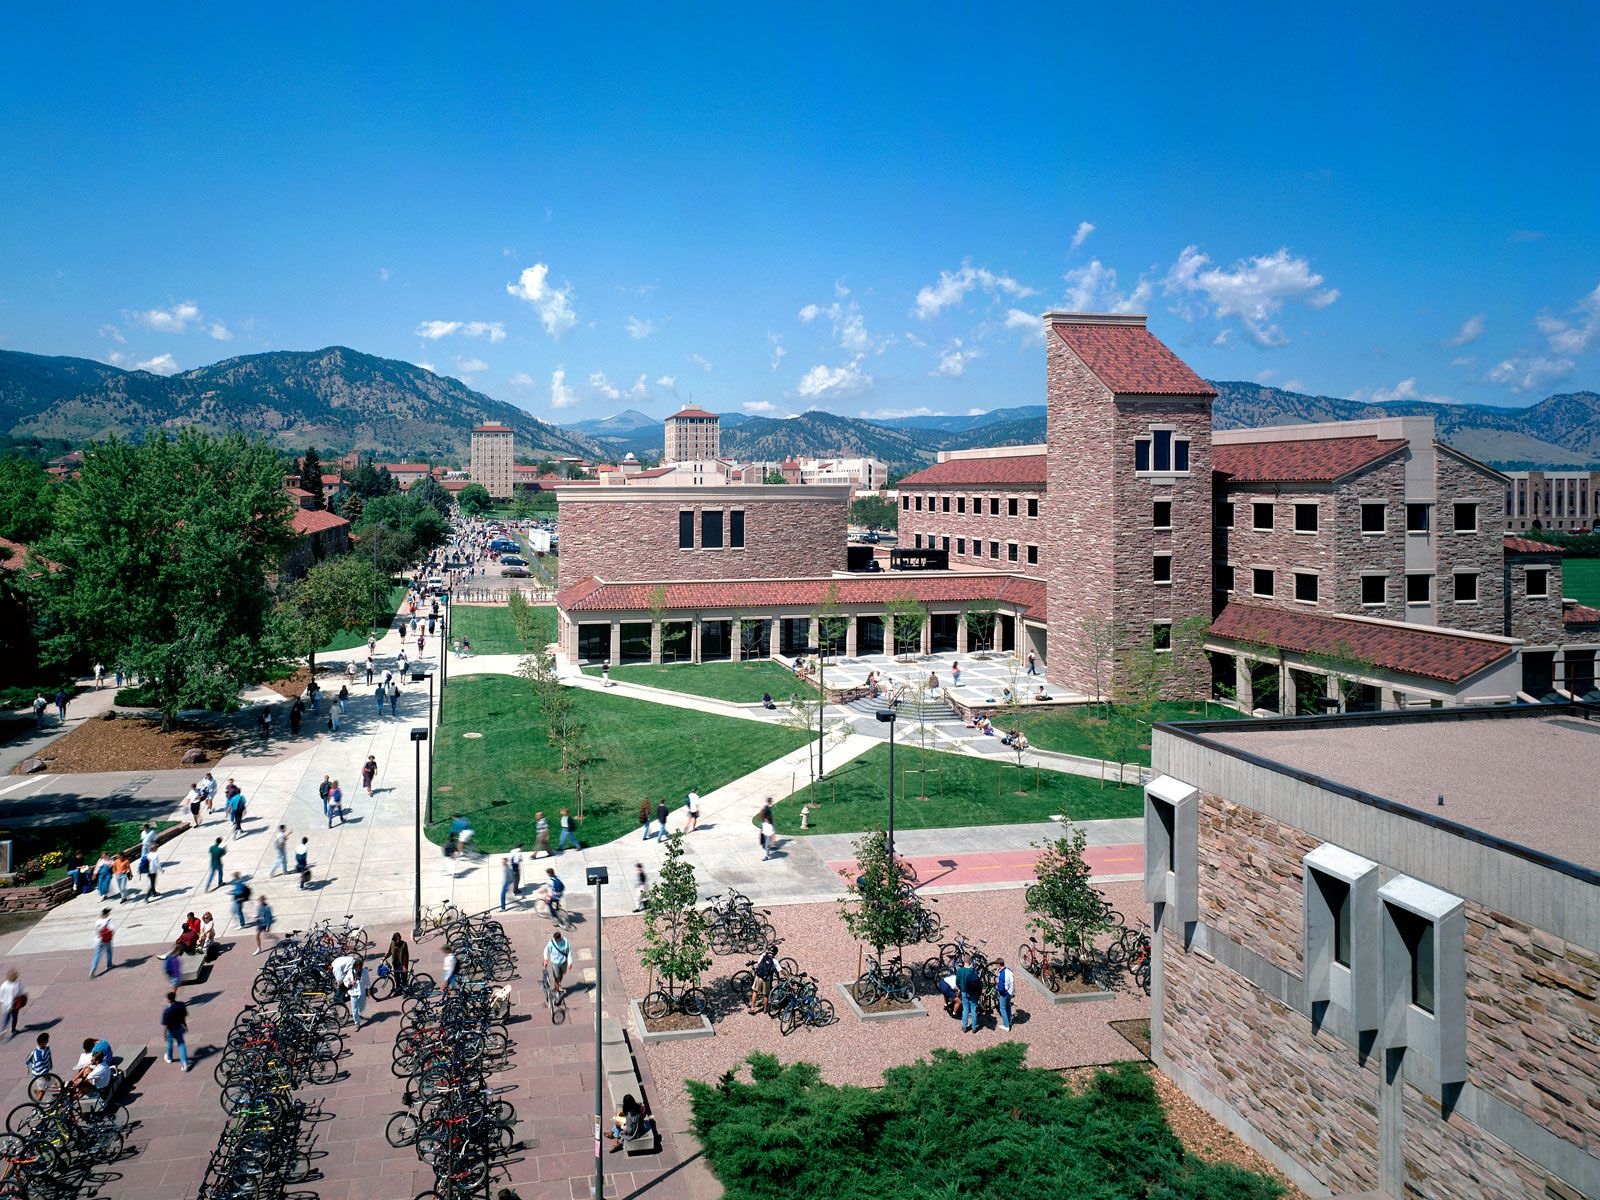
\includegraphics[width=\textwidth]{images/test01}
	\end{subfigure}
	\par\bigskip
	\begin{subfigure}[h]{0.6\textwidth}
		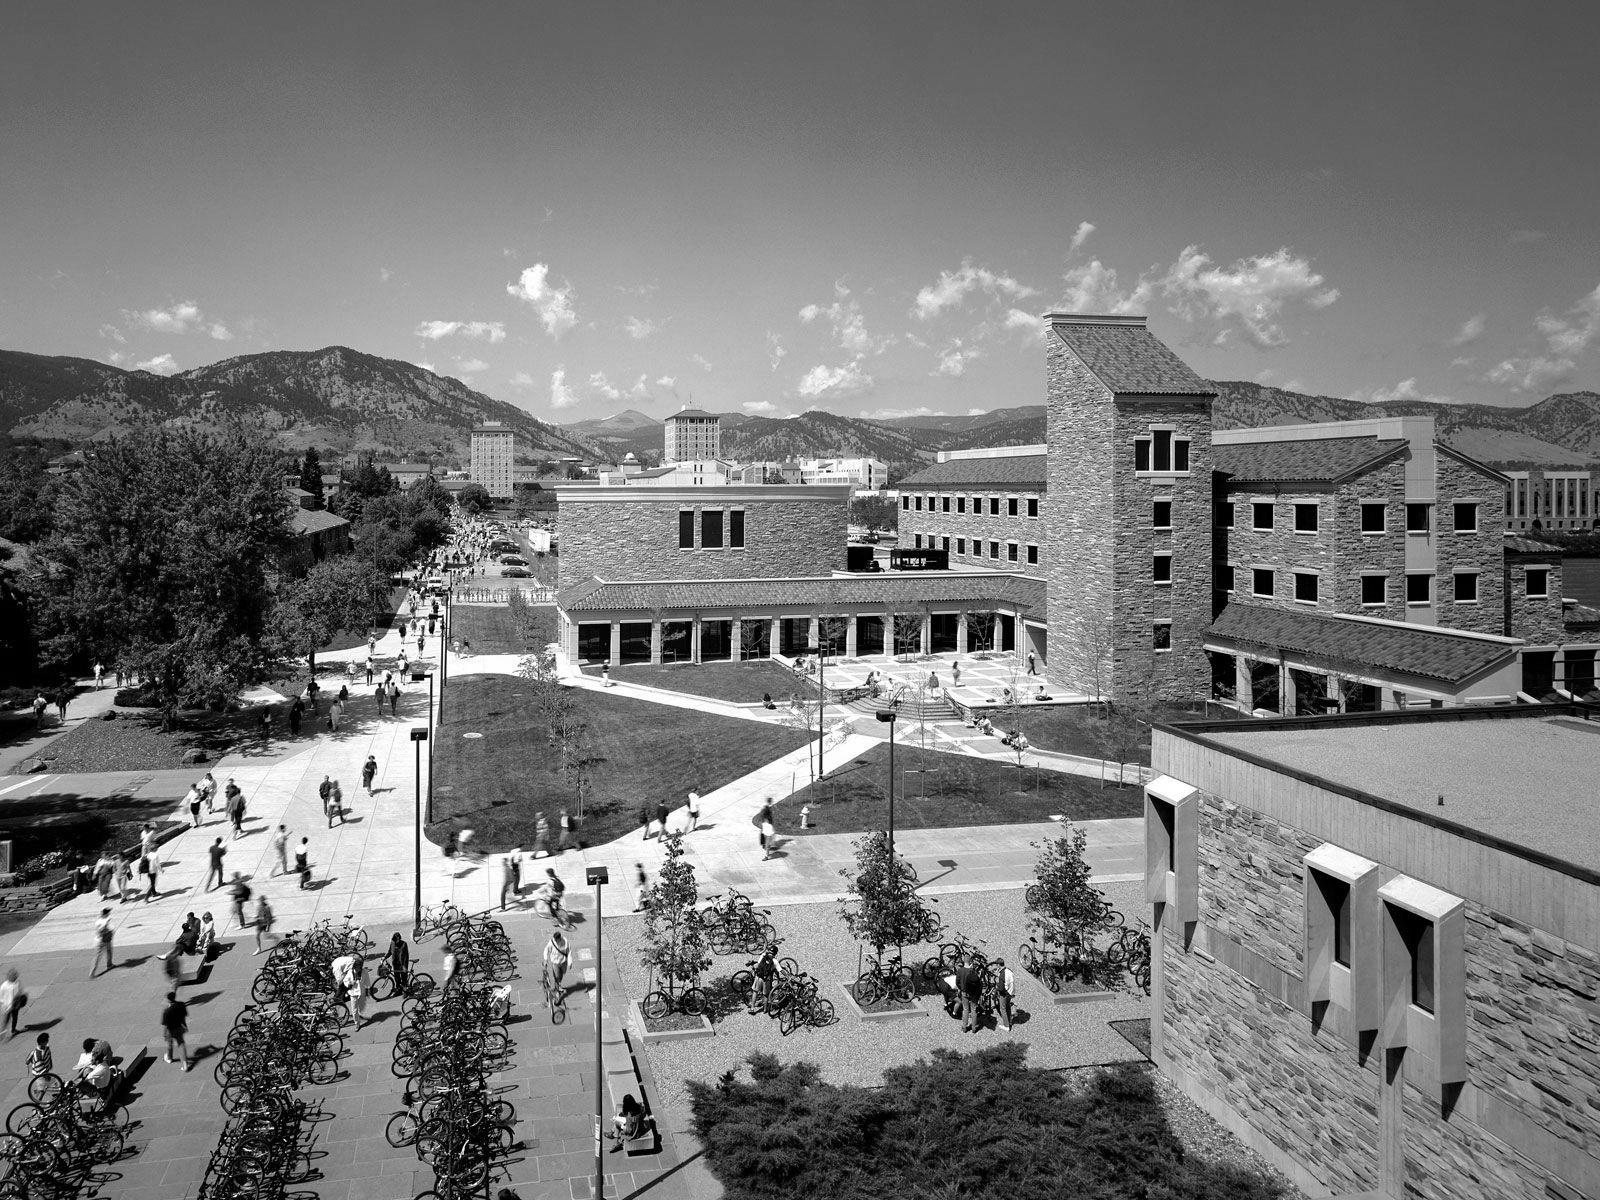
\includegraphics[width=\textwidth]{figs/test01_gray}
	\end{subfigure}
\end{figure}

\pagebreak

\tableofcontents

\pagebreak

\addcontentsline{toc}{section}{Introduction}
\section{Introduction}
In this discussion, we will be exploring some common manipulations applied to images as an introduction to image processing. The analysis will be performed in Python, using a few libraries such as \verb|Pillow| for basic image file manipulations (opening, saving), \verb|numpy| for efficient array operations, \verb|scipy.signal| for some Fourier functionality, \verb|scipy.interpolate| for interpolation, \\ \verb|collections.Counter| to count occurrences of multiple values in a list, and \verb|matplotlib.pyplot| for basic plotting. We will use functions from these libraries to help perform grayscale conversion, contrast enhancement, edge detection, and image resizing, although most of the code for these will be developed from scratch.

\addcontentsline{toc}{subsection}{Background}

\subsection{Background}
We will be working with a common uncompressed image format, BMP (short for bitmap). This file type begins with a short header, followed by a 2-dimensional array of pixel information. Color BMP files store three 8-bit numbers for each pixel, corresponding to an R, G, and B intensity value.

\begin{figure}[ht]
	\centering
	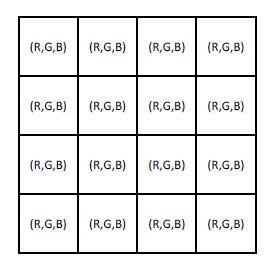
\includegraphics[width=0.5\textwidth]{figs/rgb_example}
	\caption{Example of a 4x4 color BMP image file}
	\label{fig:rgb_example}
\end{figure}

Different combinations of the three chroma values produce unique colors. Given 8-bit color depth, it is possible to represent $2^{24}$ colors.
In this lab, we will only be processing monochromatic (grayscale) images, with only 8 bits per pixel (0=black, 255=white). This will simplify analysis. The monochrome value associated with a pixel can be found from its RGB values using a dot product

\begin{equation} \label{eq:Y}
Y = (0.299,0.587,0.114)\cdot(R,G,B)
\end{equation}

The BMP header encodes image size and some other metadata. We will use \verb|Pillow| to import and export images in Python. \verb|Pillow| basically converts the input image to a BMP format when \verb|open()| is called.

\pagebreak

\section{Grayscale Conversion}
\subsection{Introduction} 
In many image processing tasks, color is unnecessary. Converting between color spaces (there are more than just grayscale and RGB) can be done using a matrix multiplication. YUV is a common matrix to use, found in TV applications (Y represents luminosity).

\begin{equation}\label{eq:YUV}
     \begin{bmatrix}
       Y \\
       U \\
       V
     \end{bmatrix}
     =
     \begin{bmatrix}
       0.299 & 0.587 & 0.114 \\
       -0.14713 & -0.28886 & 0.436 \\
       0.615 & -0.51499 & -0.10001
     \end{bmatrix}
     \begin{bmatrix}
       R \\
       G \\
       B
     \end{bmatrix}
\end{equation}

U and V are color difference signals and can be positive or negative, while Y ranges from 0 to 255.

\subsection{Method} 
We will use \verb|Pillow| for image input/output in Python. Importing an image will also involve converting it into a \verb|numpy| array for processing. The basic implementation is to open the file, convert it to a \verb|numpy| array, take the dot product of the Y vector and the image (as in eq. \ref{eq:Y}), and clip out-of-range values. See \ref{app:gray} for the full implementation.

\subsection{Results} 
Two images before and after grayscale conversion are shown below. 

\begin{figure}[ht]
	\centering
	\begin{subfigure}[h]{0.45\textwidth}
		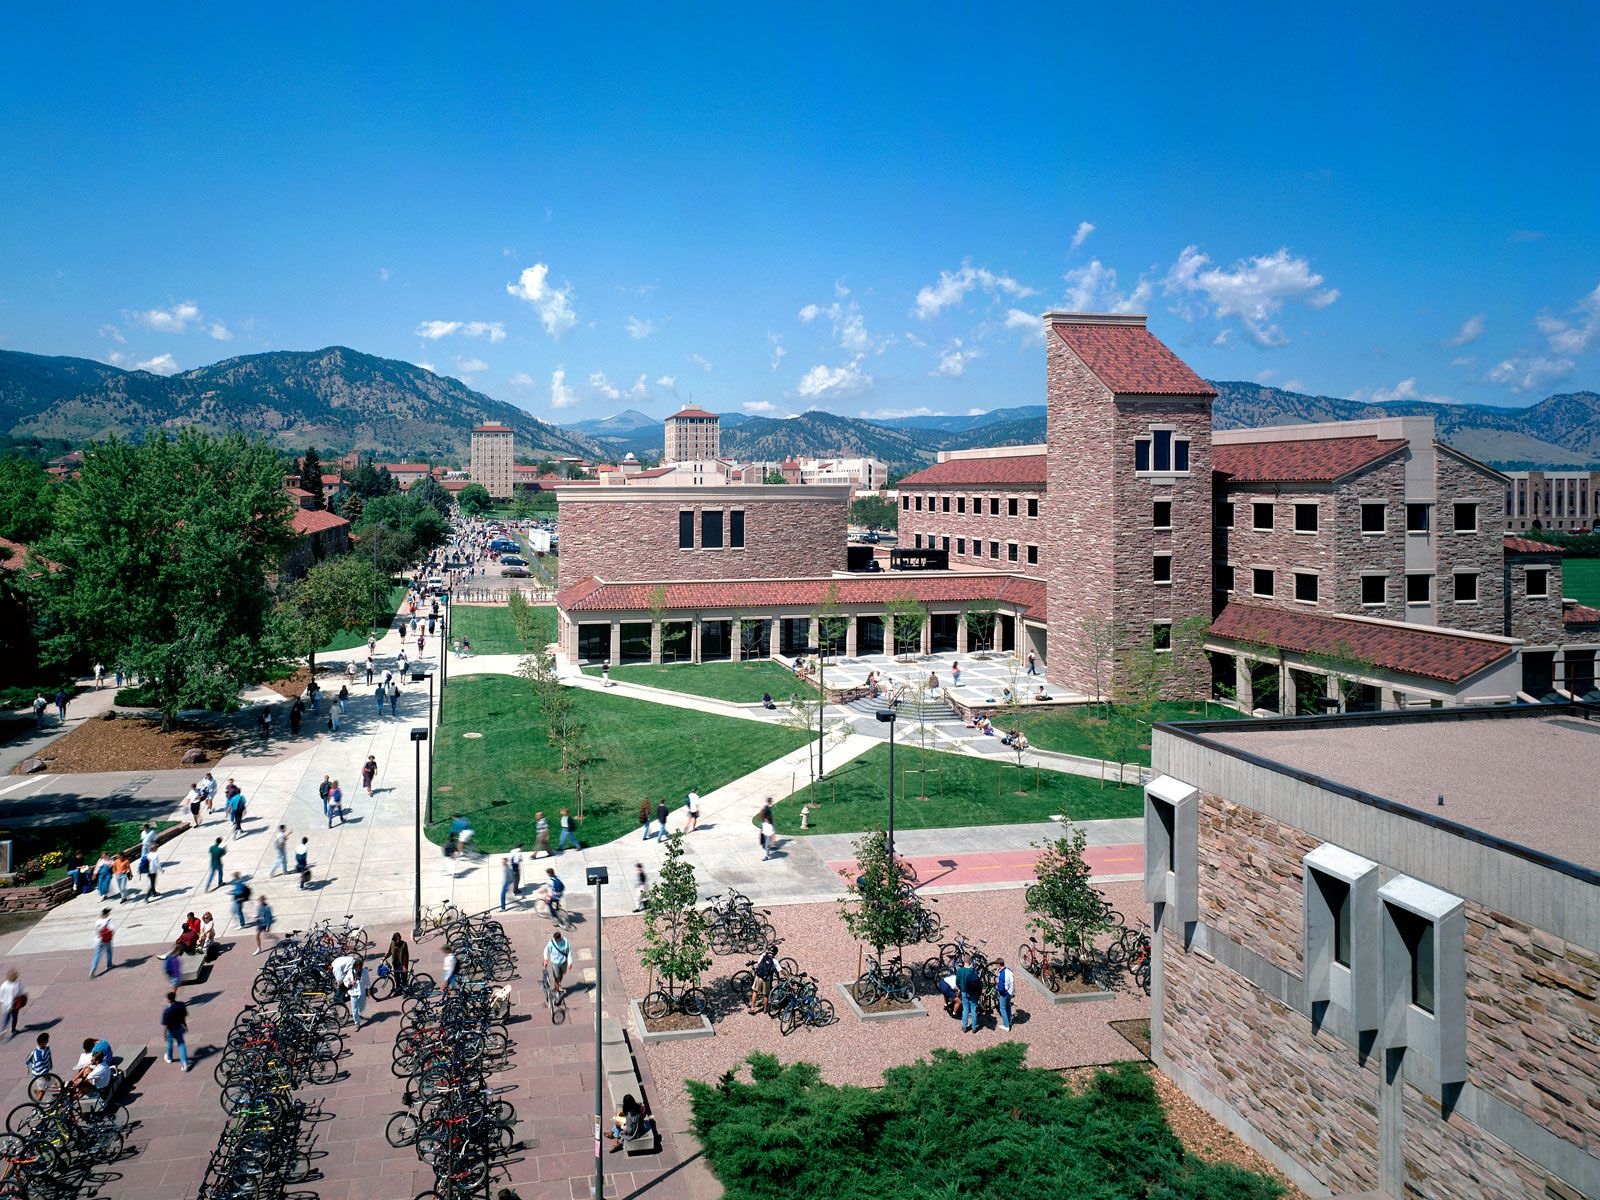
\includegraphics[width=\textwidth]{images/test01}
		\caption{Before}
		\label{fig:gray1_bef}
	\end{subfigure}
	\begin{subfigure}[h]{0.45\textwidth}
		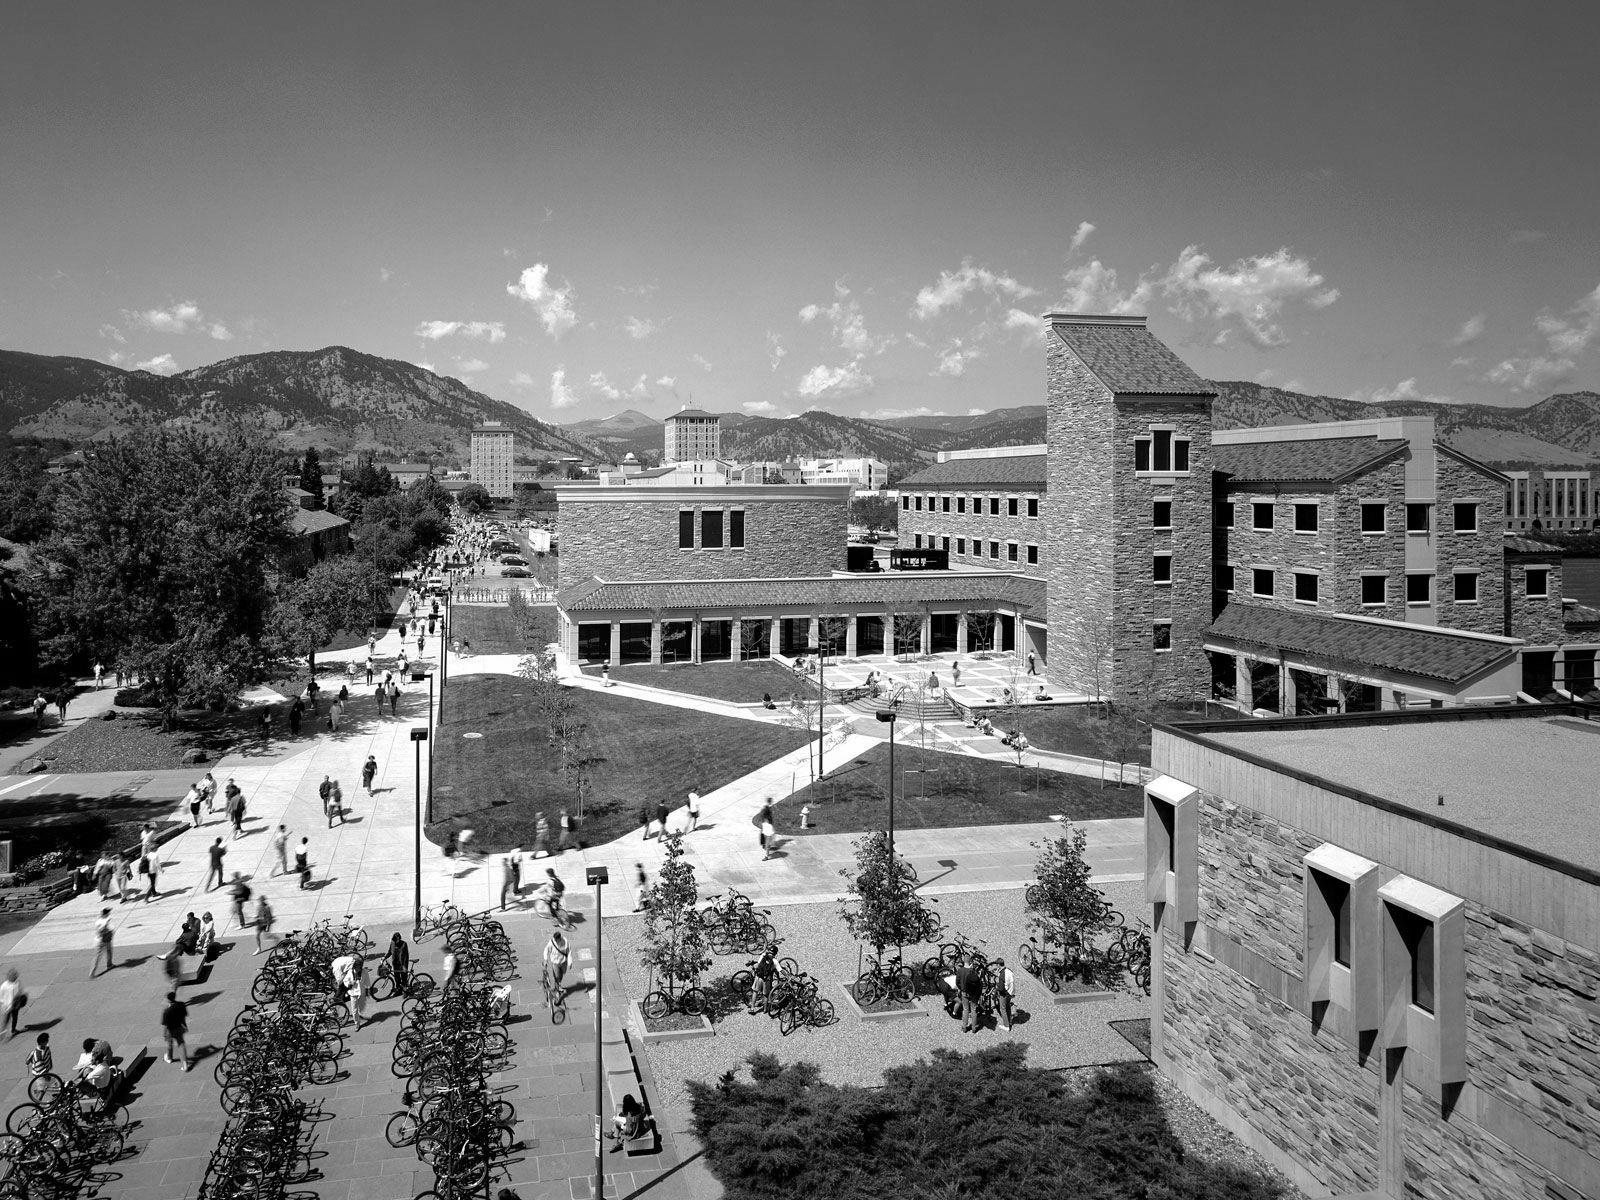
\includegraphics[width=\textwidth]{figs/test01_gray}
		\caption{After}
		\label{fig:gray1_aft}
	\end{subfigure}
	\caption{A picture of the Math building on CU Boulder campus before and after grayscale conversion.}
	\label{fig:gray1}
\end{figure}

\begin{figure}[ht]
	\centering
	\begin{subfigure}[h]{0.45\textwidth}
		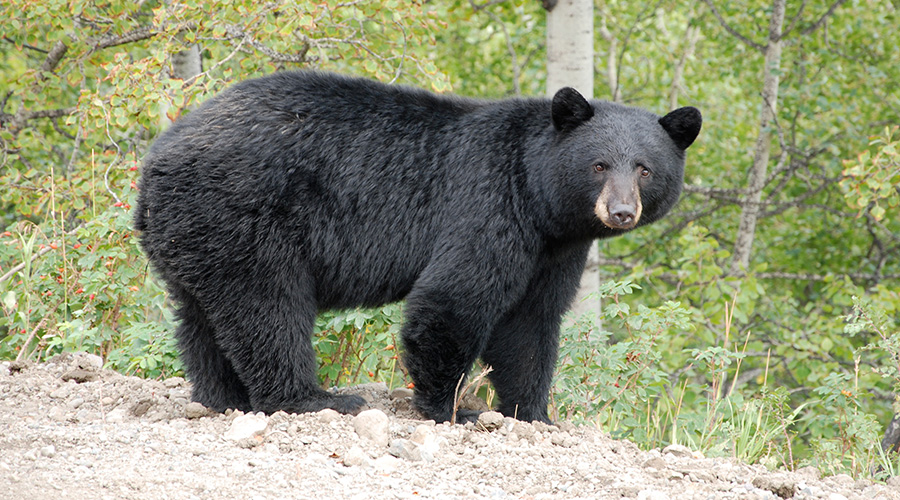
\includegraphics[width=\textwidth]{images/test02}
		\caption{Before}
		\label{fig:gray2_bef}
	\end{subfigure}
	\begin{subfigure}[h]{0.45\textwidth}
		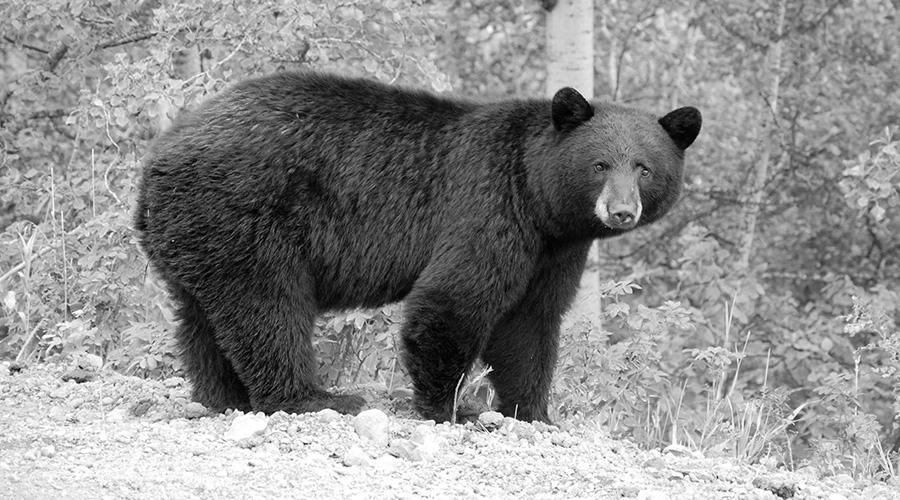
\includegraphics[width=\textwidth]{figs/test02_gray}
		\caption{After}
		\label{fig:gray2_aft}
	\end{subfigure}
	\caption{A picture of a bear before and after grayscale conversion.}
	\label{fig:gray2}
\end{figure}

\clearpage

\section{Contrast Enhancement}

\subsection{Introduction}
Sometimes a picture will have low dynamic range and appears low contrast. A simple contrast enhancement process based on \textit{histogram equalization} can make a huge improvement. In this part of the lab, we will be implementing histogram equalization as a contrast enhancement algorithm. This means that we will take an image with tightly grouped intensities and try to 'equalize' it so that the intensities are evenly distributed.

\subsection{Method} 
We begin by opening an image and converting it to grayscale, using the \verb|Pillow| function, \verb|convert('L')|. Then, we can use \verb|collections.Counter| to find the number of occurrences of each intensity value. \verb|Counter| returns an array of the values, but is structured like a dictionary and is not sorted. Thus, looping over intensity (0 to 255) we can extract the frequencies in a sorted \verb|numpy| array.

\begin{lstlisting}[language=Python]
image = image.convert('L')
image = np.asarray(image, np.float)
hist_before = np.zeros(256, dtype=int)
freq = Counter(np.reshape(image, image.shape[0] * image.shape[1]))
for p in range(256):
    hist_before[p] = freq[p]
\end{lstlisting}

At this point, \verb|hist_before| holds a histogram of intensity.

\begin{figure}[ht]
	\centering
	\begin{subfigure}[h]{0.45\textwidth}
		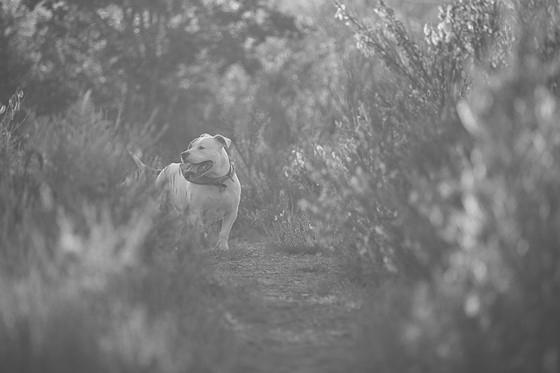
\includegraphics[width=\textwidth]{figs/lc1_gray}
		\caption{A low-contrast image.}
		\label{fig:gray_lc1}
	\end{subfigure}
	\begin{subfigure}[h]{0.45\textwidth}
		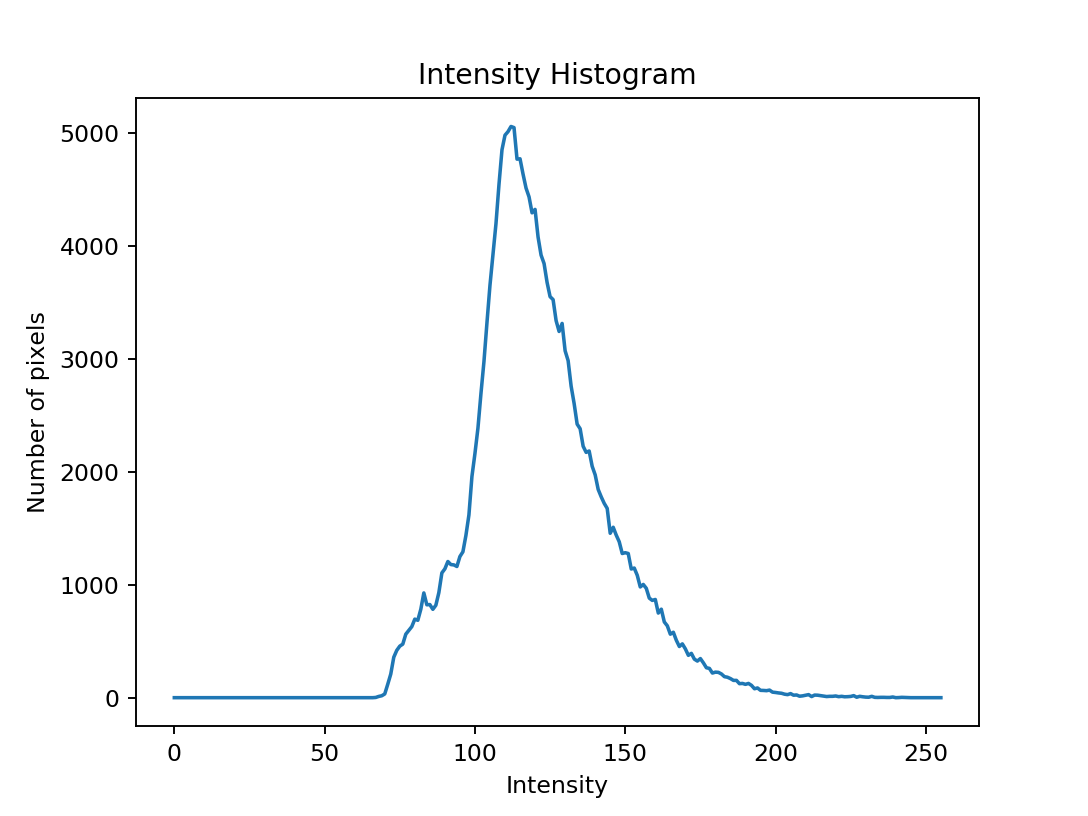
\includegraphics[width=\textwidth]{figs/lc1_hist_bef}
		\caption{Intensity histogram.}
		\label{fig:lc1_hist_bef}
	\end{subfigure}
	\caption{Intensity histogram of a low contrast image. Note the lack of any values on the low or high end of the spectrum. This is what makes it low contrast, as there is low dynamic range.}
	\label{fig:lc1_hist}
\end{figure}

Next, we want to find a function to map intensities of one value to another in a way that will "equalize" the histogram in figure \ref{fig:lc1_hist_bef}.
We wish to remap the intensities of the original image, so that each intensity occurs with the same frequency. Then the ideal pixel count for any given intensity would be $P = (\text{total \# of pixels}) / (\text{number of intensity values})$. We will ignore values of 0 or 255 as they cannot be remapped to anything except themselves. Looping over intensity (1 to 254), we hold a running sum, counting the number of pixels that have been remapped in a variable \verb|curr_sum|. Initially, we find pixels to be remapped to a value of 1. We do this until we've remapped at least as many pixels as we had aimed for. Then, we start mapping to a new value, determined by \verb|round(curr_sum/P)|, which accounts for some overshoot.

\pagebreak

\begin{lstlisting}[language=Python]
remap = np.zeros(256, dtype=int)
remap[-1] = 255
histSum = sum(hist_before[1:-2])
P = histSum / 254
T = P
outval = 1
curr_sum = 0
# build remap table
for inval in range(1, 255, 1):
    curr_sum += hist_before[inval]
    remap[inval] = outval
    if (curr_sum > T):
        outval = round(curr_sum/P)
        T = outval*P
\end{lstlisting}

\begin{figure}[ht]
	\centering
	\begin{subfigure}[h]{0.45\textwidth}
		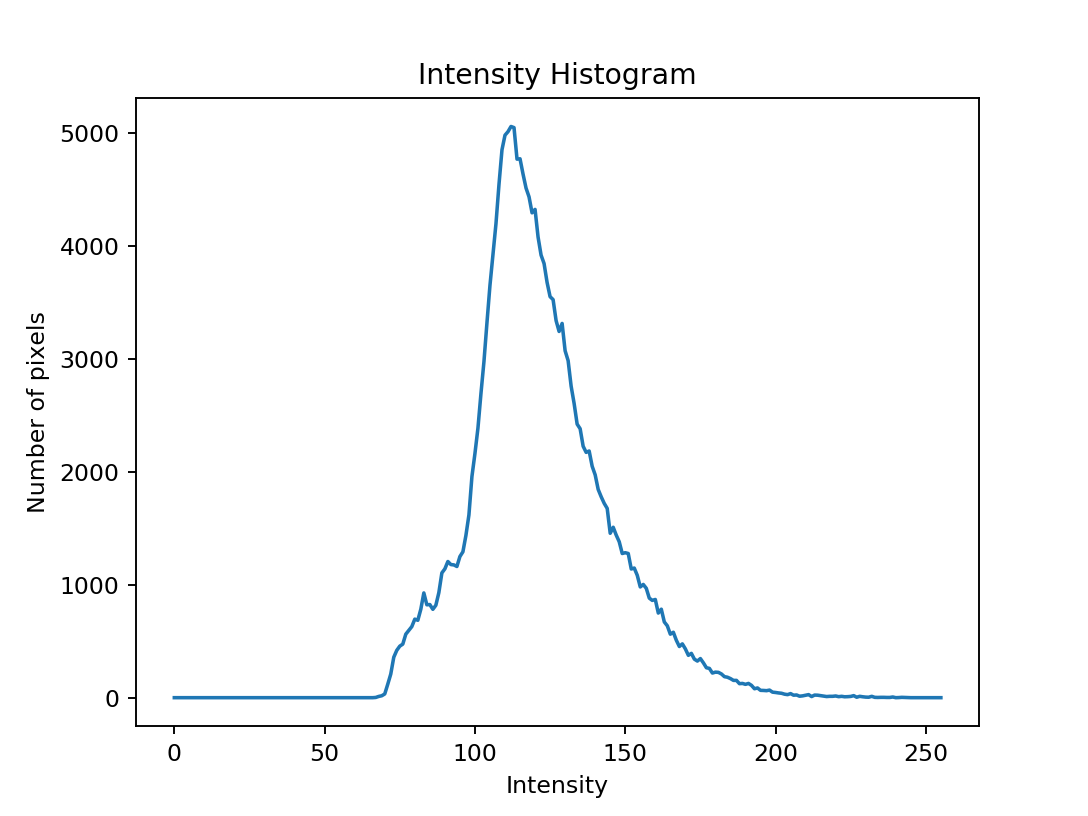
\includegraphics[width=\textwidth]{figs/lc1_hist_bef}
		\caption{Histogram of low-contrast image}
		\label{fig:lc1_hist_before_r}
	\end{subfigure}
	\begin{subfigure}[h]{0.45\textwidth}
		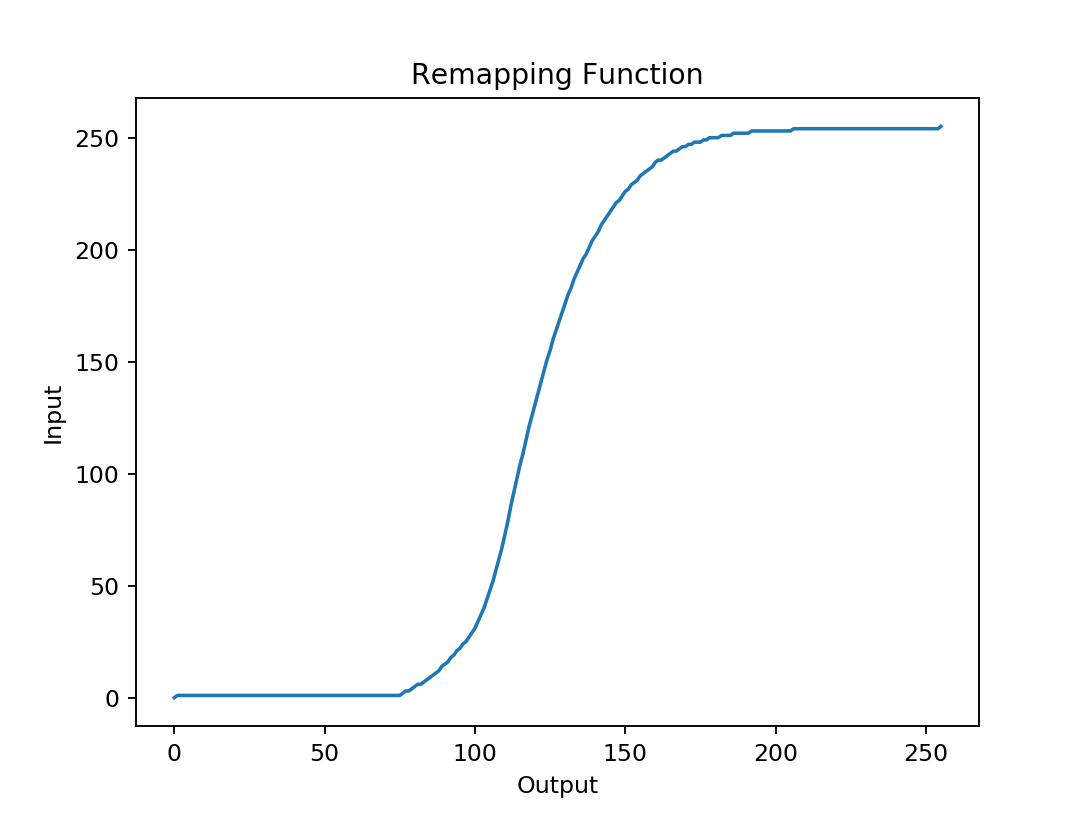
\includegraphics[width=\textwidth]{figs/lc1_remap}
		\caption{Remapping function}
		\label{fig:lc1_remap}
	\end{subfigure}
	\caption{Histogram and remapping function for a low contrast image.}
	\label{fig:lc1_remap_func}
\end{figure}

Figure \ref{fig:lc1_remap} shows how intensity values are remapped for the image in \ref{fig:gray_lc1}. Notice that many of the pixel intensities centered around the middle will be spread out to occupy most of the spectrum.
Next, we need to apply the remapping function to the image and produce the contrast-enhanced picture. To do this, we will use \verb|numpy.where|.

\begin{lstlisting}[language=Python]
image_equalized = np.zeros_like(image)
for intensity in range(256):
    image_equalized = np.where(image == intensity, remap[intensity], image_equalized)
\end{lstlisting}

\pagebreak

\subsection{Results}
The full results of contrast enhancement for two images can be seen in figures \ref{fig:eq1} and \ref{fig:eq2}.

\begin{figure}[ht]
	\ContinuedFloat*
	\centering
	\begin{subfigure}[h]{0.7\textwidth}
		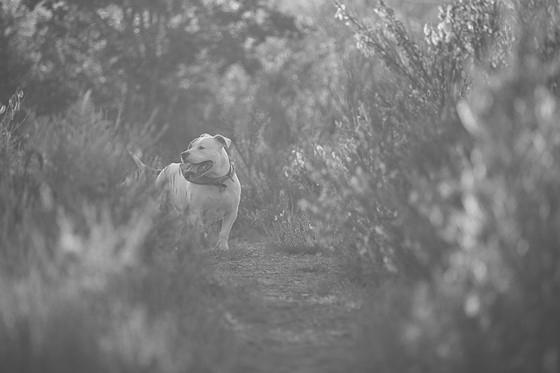
\includegraphics[width=\textwidth]{figs/lc1_gray}
		\caption{Original}
		\label{fig:lc1_orig}
	\end{subfigure}
	\par\bigskip
	\begin{subfigure}[h]{0.75\textwidth}
		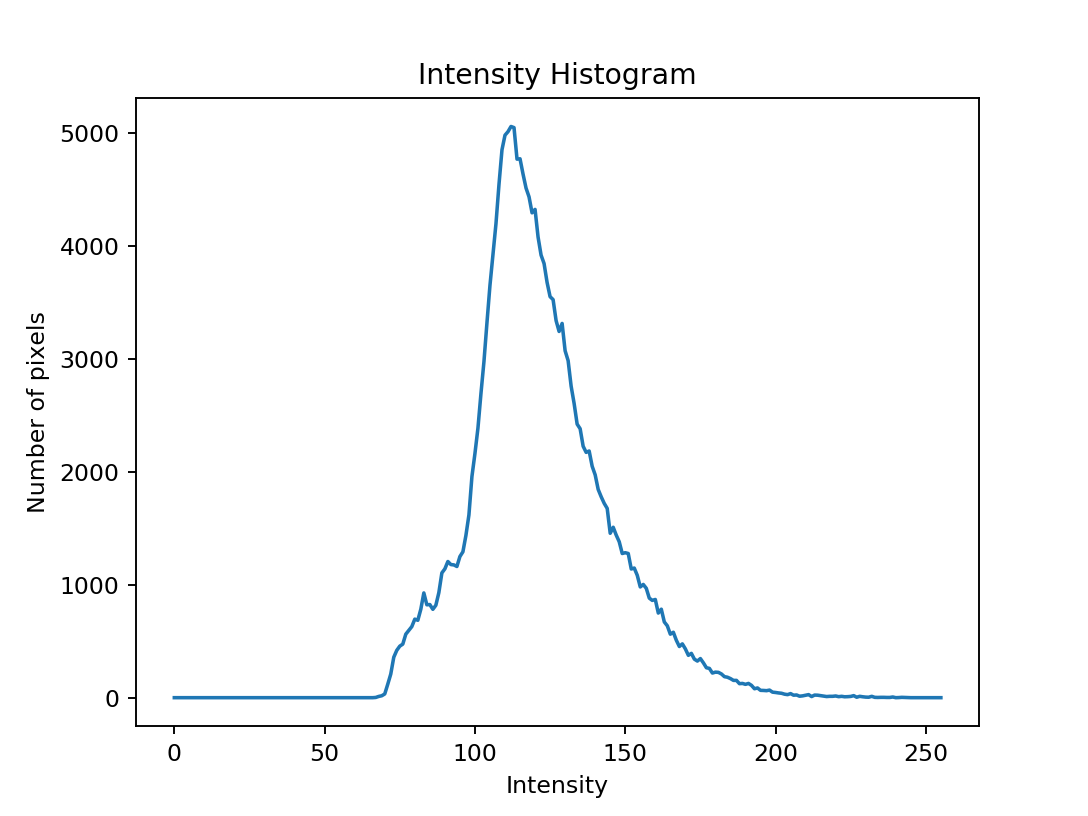
\includegraphics[width=\textwidth]{figs/lc1_hist_bef}
		\caption{Before}
		\label{fig:hist_bef_1}
	\end{subfigure}
	
	\caption{Contrast enhancement.}
	\label{fig:eq1}
\end{figure}

\clearpage

\begin{figure}[ht]
	\ContinuedFloat
	\centering
	\begin{subfigure}[h]{0.7\textwidth}
		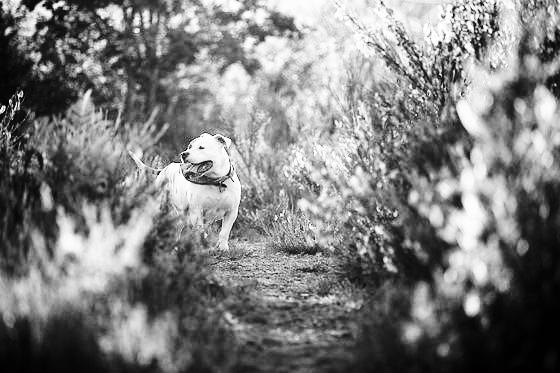
\includegraphics[width=\textwidth]{figs/lc1_ce}
		\caption{Contrast enhanced}
		\label{fig:lc1_after}
	\end{subfigure}
	\par\bigskip
	\begin{subfigure}[h]{0.75\textwidth}
		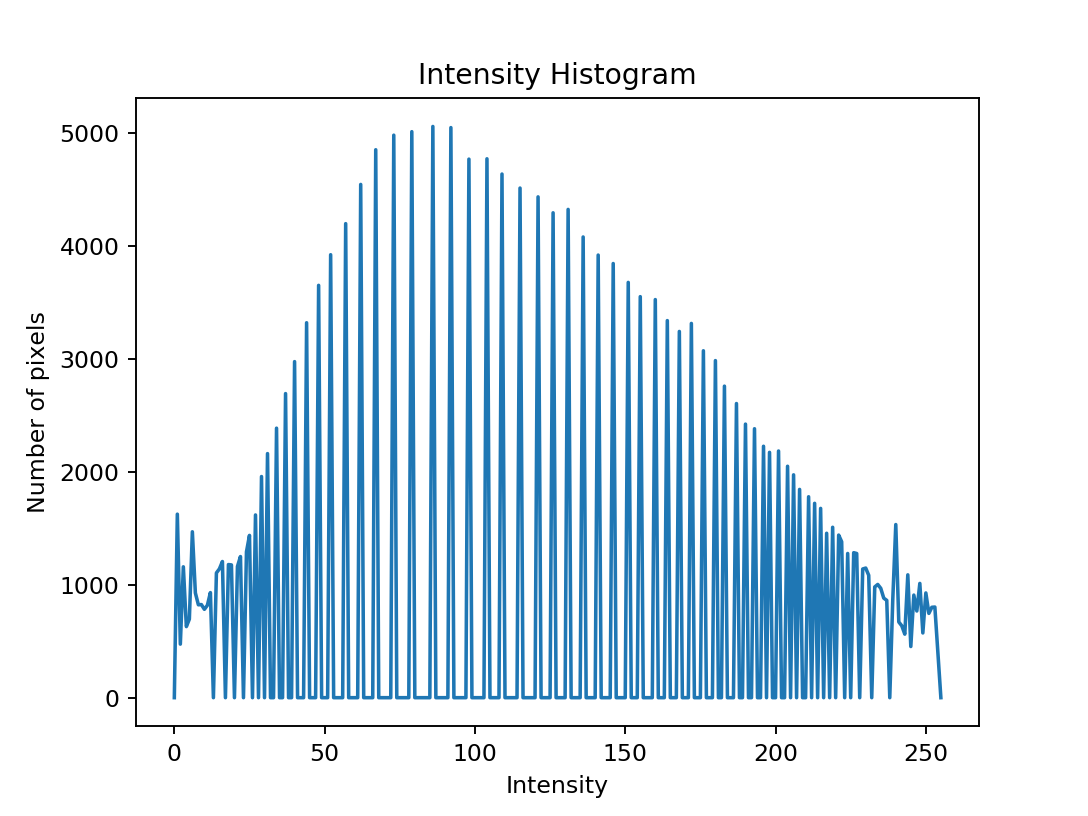
\includegraphics[width=\textwidth]{figs/lc1_hist_aft}
		\caption{After}
		\label{fig:hist_aft_1}
	\end{subfigure}
\end{figure}

Figure \ref{fig:eq1} shows the process of histogram equalization for a picture of a dog. Obviously the original image could use some improvement and the histogram in \ref{fig:hist_bef_1} indicates why. The histogram has been improved so there's a lot more dynamic range, shown in fig. \ref{fig:hist_aft_1}, but the processed image in fig. \ref{fig:lc1_after} is oversaturated. It's better than before and has much more dynamic range, but this is a poor result for improving the quality of an image.

\clearpage

\begin{figure}[ht]
	\ContinuedFloat*
	\centering
	\begin{subfigure}[h]{0.7\textwidth}
		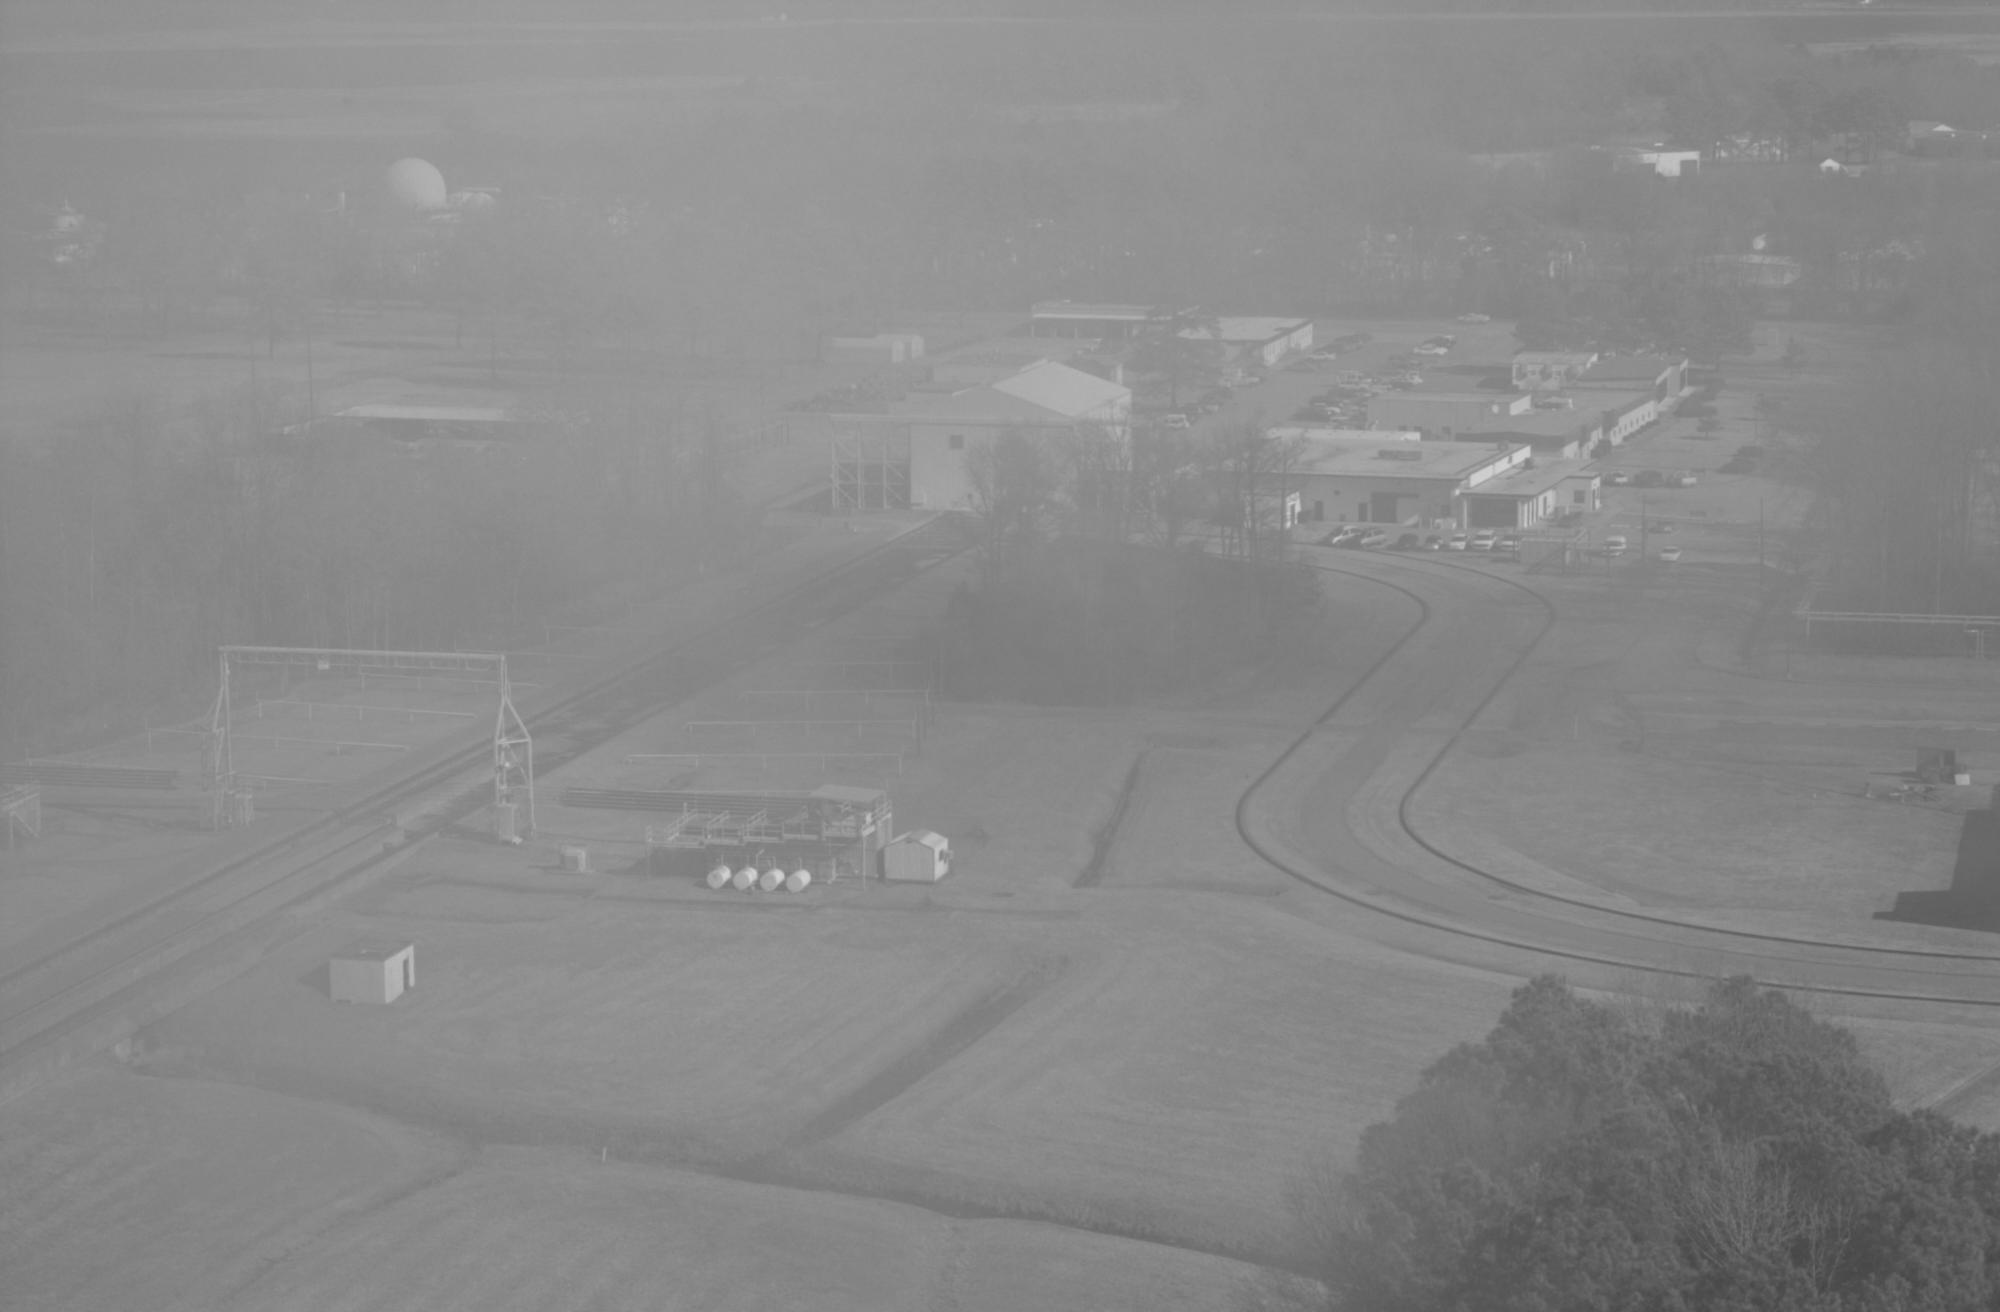
\includegraphics[width=\textwidth]{figs/lc2_gray}
		\caption{Original}
		\label{fig:lc2_orig}
	\end{subfigure}
	\par\bigskip
	\begin{subfigure}[h]{0.75\textwidth}
		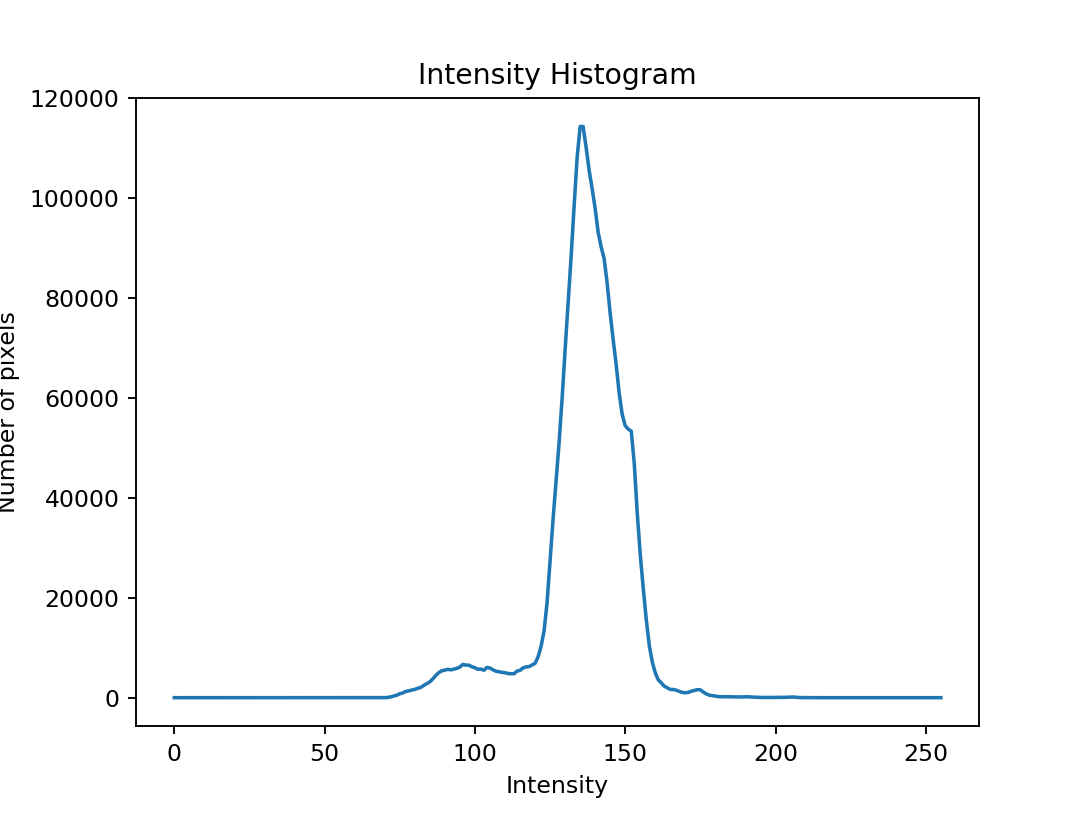
\includegraphics[width=\textwidth]{figs/lc2_hist_bef}
		\caption{Before}
		\label{fig:hist_bef_2}
	\end{subfigure}
	
	\caption{Contrast enhancement.}
	\label{fig:eq2}
\end{figure}

\clearpage

\begin{figure}[ht]
	\ContinuedFloat
	\centering
	\begin{subfigure}[h]{0.7\textwidth}
		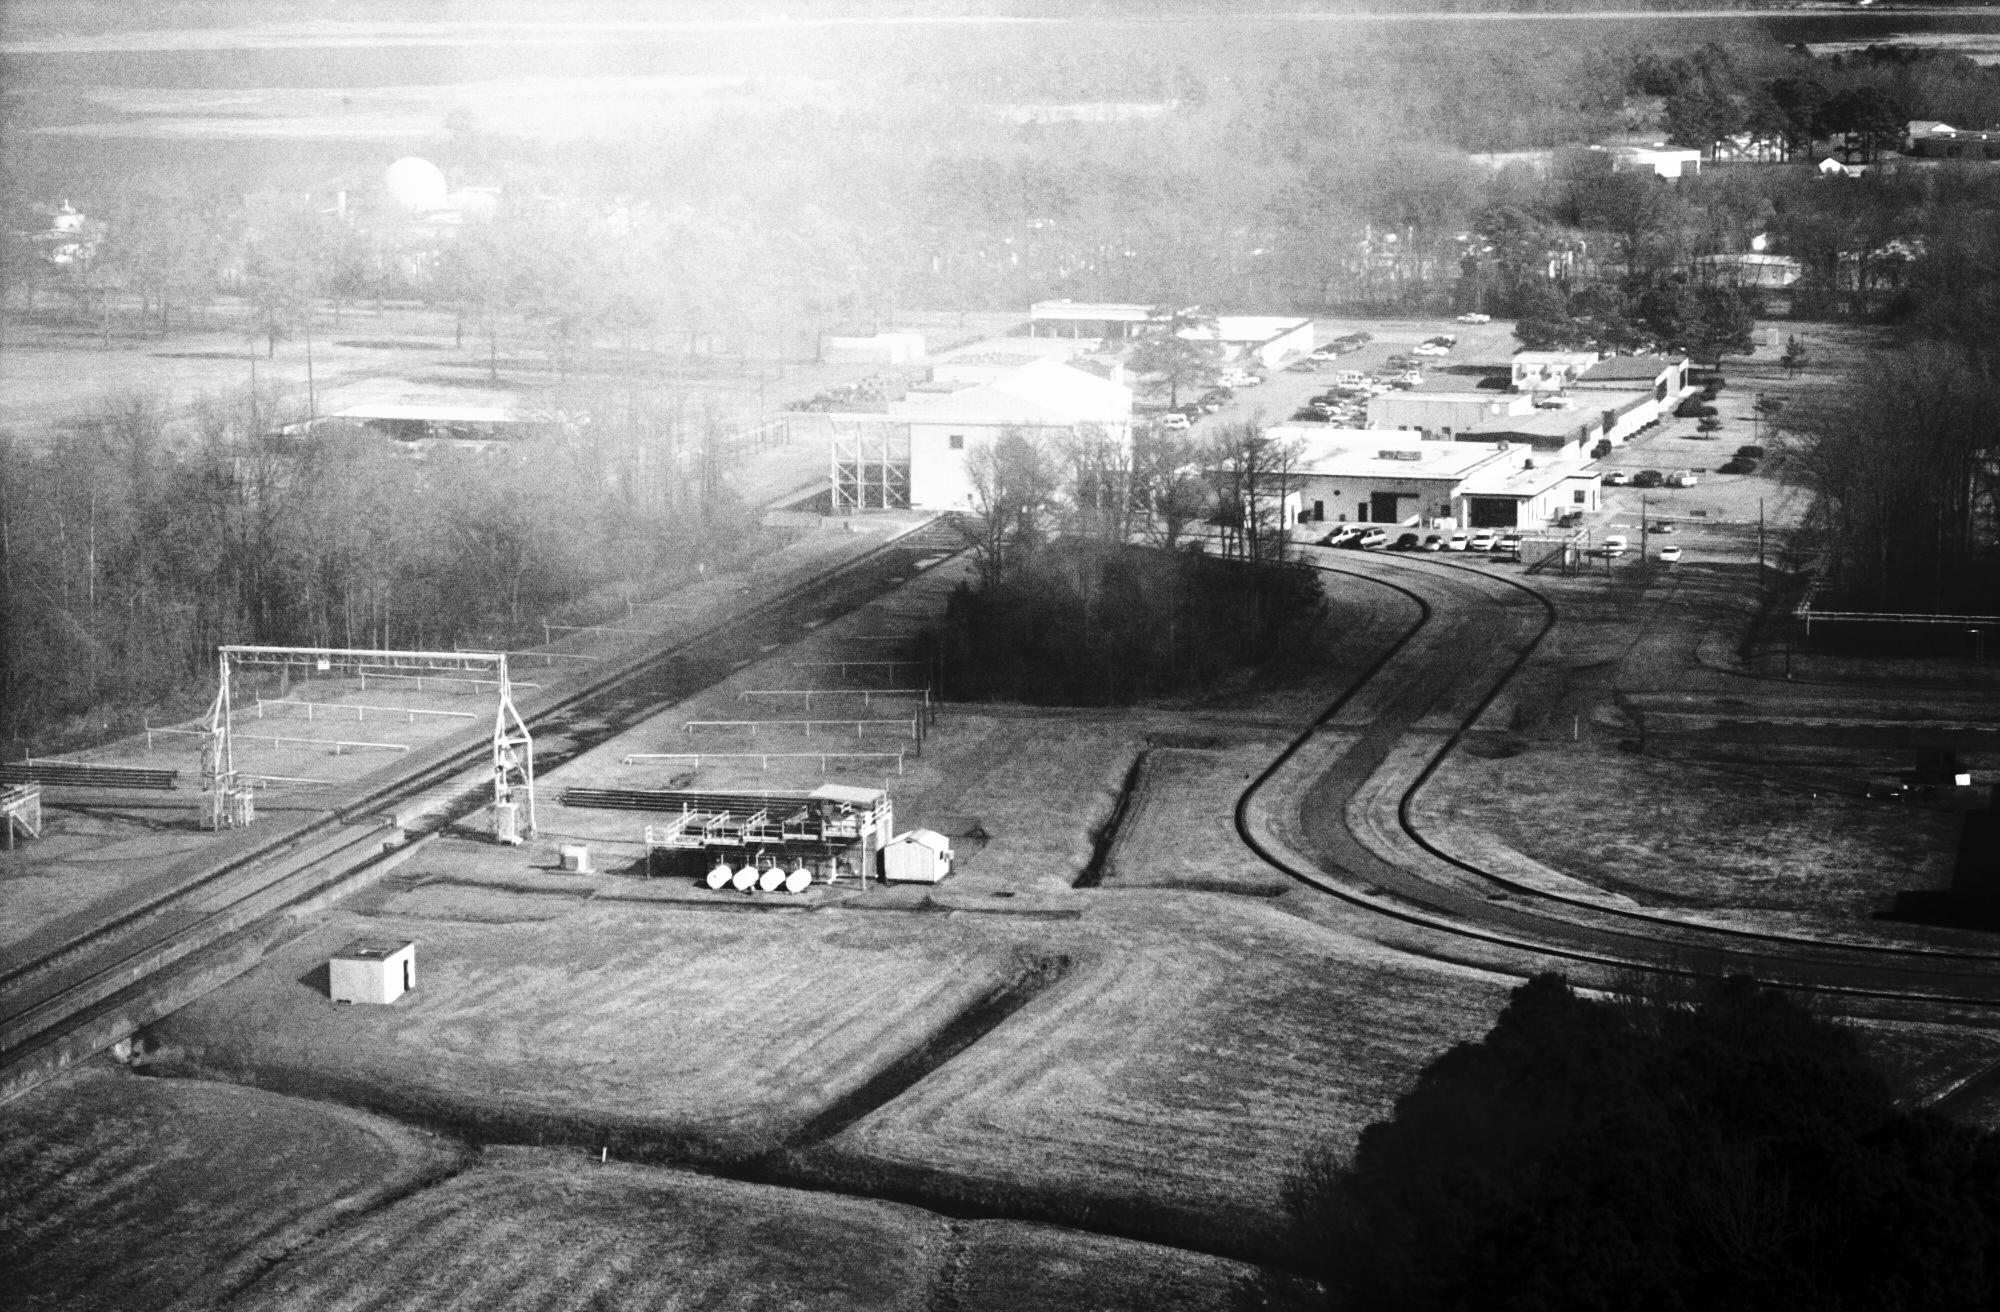
\includegraphics[width=\textwidth]{figs/lc2_ce}
		\caption{Contrast enhanced}
		\label{fig:lc2_after}
	\end{subfigure}
	\par\bigskip
	\begin{subfigure}[h]{0.75\textwidth}
		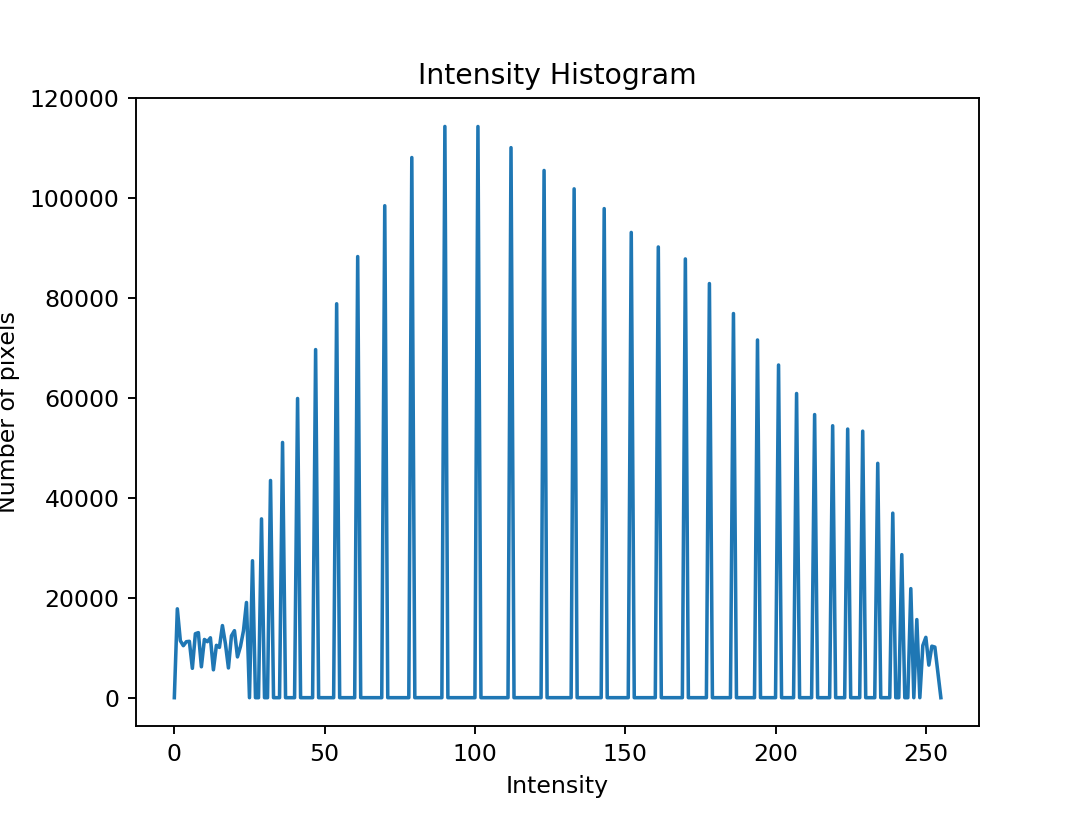
\includegraphics[width=\textwidth]{figs/lc2_hist_aft}
		\caption{After}
		\label{fig:hist_aft_2}
	\end{subfigure}
\end{figure}

Figure \ref{fig:eq2} again shows the equalization process for a low contrast image - this time it's a rural scene. Again, the histogram is much more spread and the image contrast has been increased. This one looks a lot more natural, albeit slightly oversaturated as well. 
Despite calling this "equalization", the histograms are not flat. I think this makes sense, since there's only so much an algorithm like this can do to spread the intensities out. I would be happy with this result. Next, we will look at a couple more, not-so-low-contrast images processed in the same way.

\clearpage

\begin{figure}[ht]
	\centering
	\begin{subfigure}[h]{0.45\textwidth}
		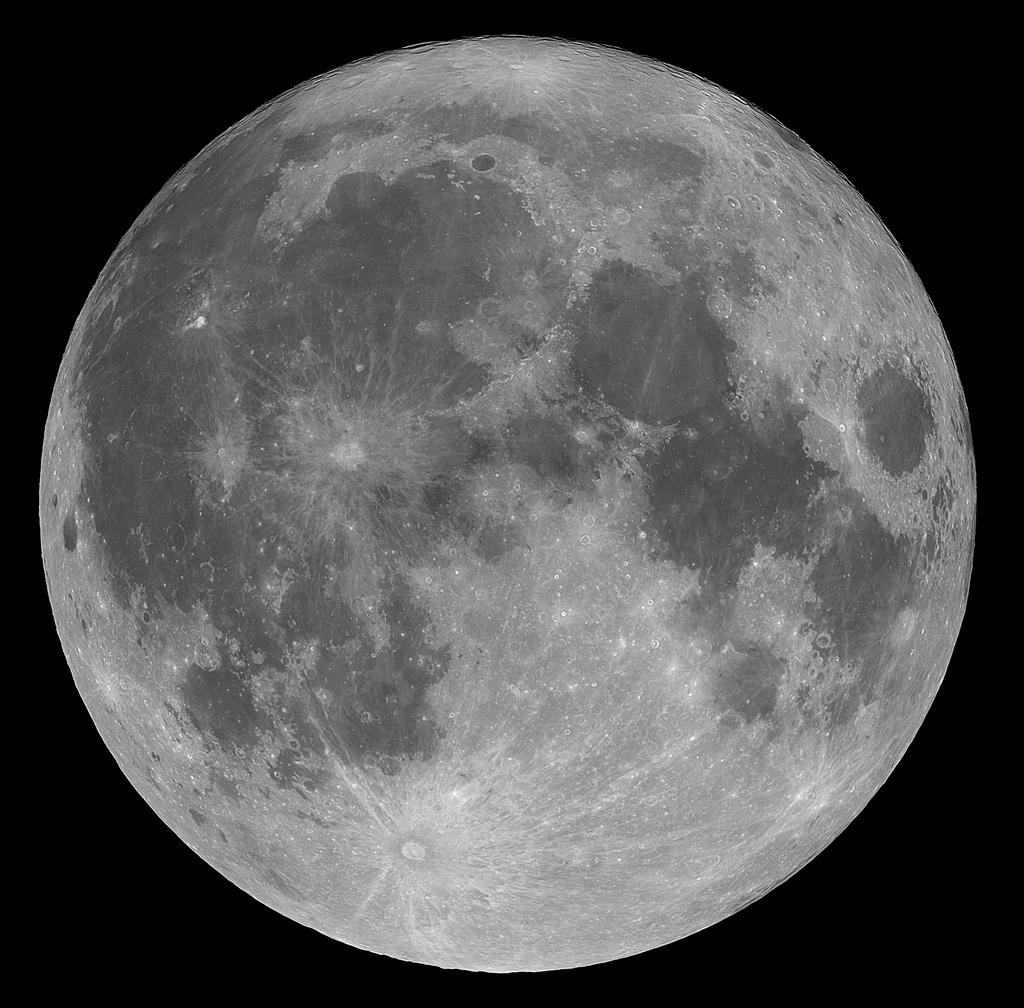
\includegraphics[width=\textwidth]{figs/lc3_gray}
		\caption{Before}
		\label{fig:moon_bef}
	\end{subfigure}
	\begin{subfigure}[h]{0.45\textwidth}
		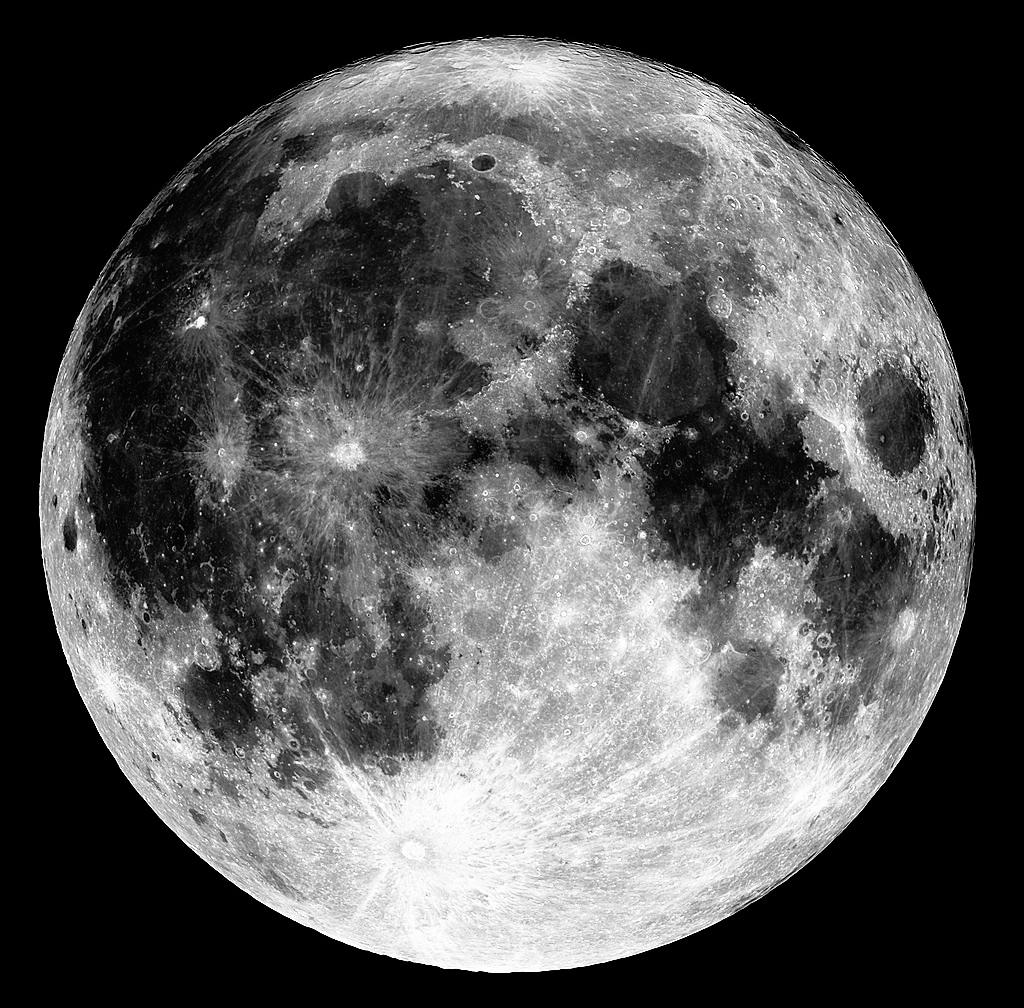
\includegraphics[width=\textwidth]{figs/lc3_ce}
		\caption{After}
		\label{fig:moon_aft}
	\end{subfigure}	
	
	\caption{Histogram equalization applied to an image with low to normal contrast.}
	\label{fig:ce_norm_moon}
\end{figure}

This picture of the moon is arguable low-contrast, but many pictures of the moon appear this way. Running the equalization algorithm on it produces an interesting result. While it may be less realistic, there is much more detail in the processed image (\ref{fig:moon_aft}).

\begin{figure}[ht]
	\centering
	\begin{subfigure}[h]{0.45\textwidth}
		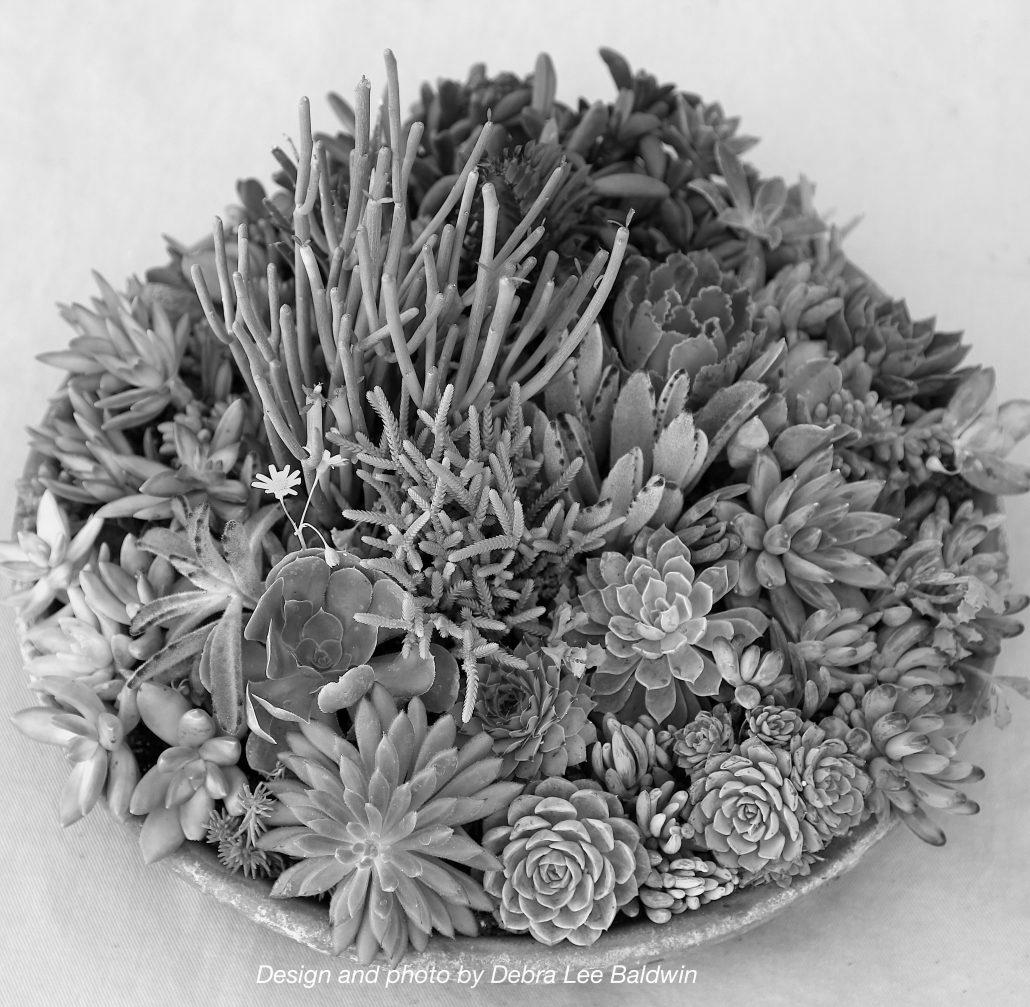
\includegraphics[width=\textwidth]{figs/succs_gray}
		\caption{Before}
		\label{fig:succs_bef}
	\end{subfigure}
	\begin{subfigure}[h]{0.45\textwidth}
		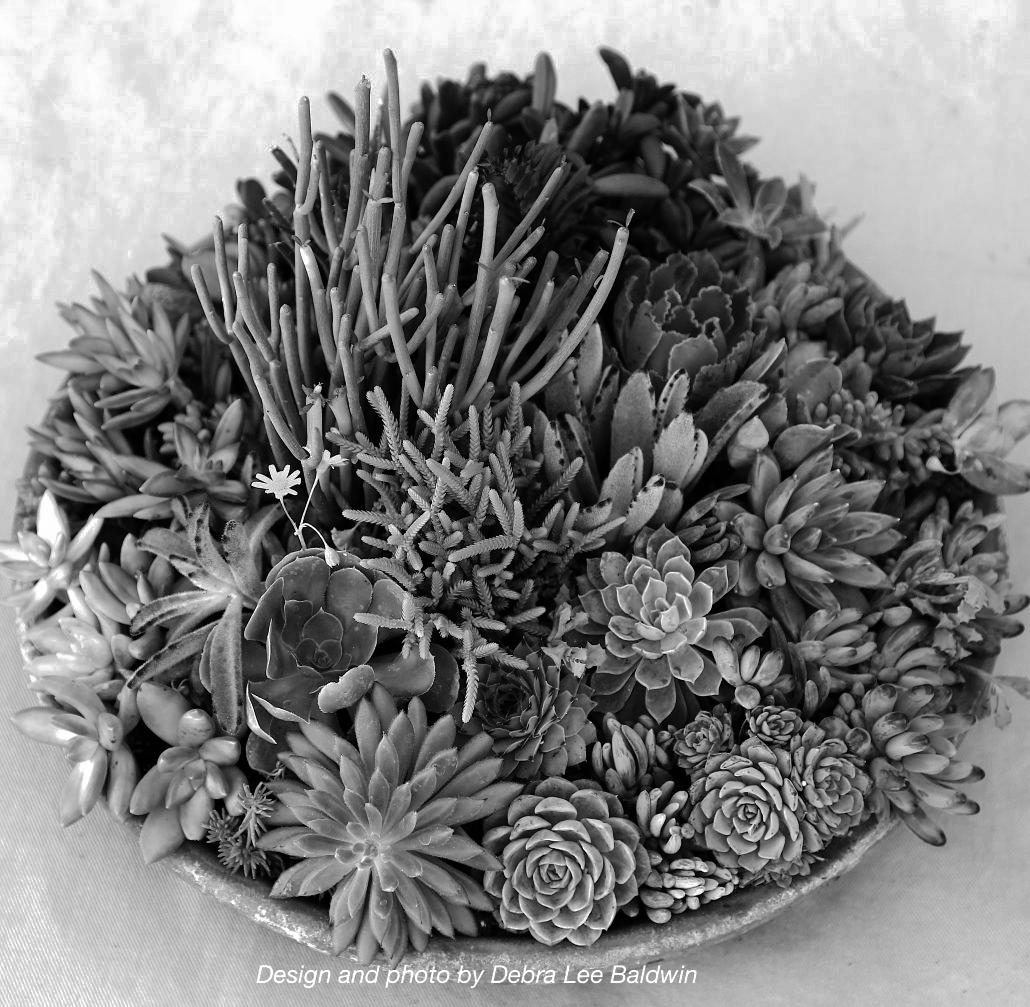
\includegraphics[width=\textwidth]{figs/succs_ce}
		\caption{After}
		\label{fig:succs_aft}
	\end{subfigure}
	
	\caption{Histogram equalization applied to an image with normal contrast.}
	\label{fig:ce_norm_succs}
\end{figure}

Figure \ref{fig:ce_norm_succs} started as a very normal image. We see in \ref{fig:succs_aft} that this algorithm boosted the contrast a bit. It looks obviously processed and the contrast is too high to look natural, but it amplified edges, so could be a good algorithm to run before edge-detection.

\textbf{Lab question 5:} This technique could be applied to color images by processing the R, G, and B channels separately.

\clearpage

\section{Sobel Edge Detection}
\subsection{Introduction}
In this part of the lab, we wish to implement an algorithm that will find the "edges" of features in an image and set those edges to maximum intensity (255). Everything else will become black (0 intnesity). Since we are processing grayscale images, we will classify rapidly changing intensity as an edge. Rapid intensity corresponds to a derivative with large magnitude at that point. If we want the derivative of intensity in our 2-D image, we need to take the partial derivatives $\frac{\partial f}{\partial x}$ and $\frac{\partial f}{\partial y}$. Then, recall the gradient of a real-valued function with N-D domain is an N-D vector pointing in the direction of maximum change. Its magnitude is the rate of change in that direction. In 2-D we have

\begin{align}
\nabla f(x,y) = \left(\frac{\partial f}{\partial x}, \frac{\partial f}{\partial y} \right) \nonumber \\
||\nabla f(x,y)||^2 = \left( \frac{\partial f}{\partial x} \right)^2 + \left( \frac{\partial f}{\partial y} \right)^2 \nonumber \\
||\nabla f|| = \sqrt{(\delta h)^2 + (\delta v)^2} \label{eq:grad}
\end{align}

\subsection{Method}
To find edges, we need to first approximate the magnitude of the gradient vector at each pixel. We will use convolution with a Sobel kernel to do this. The Sobel kernels perform both low-pass filtering and gradient estimation. We define $\frac{\partial f}{\partial x}$ and $\frac{\partial f}{\partial y}$ in the context of a 2-D image as

\begin{equation}
\frac{\partial f}{\partial x}	= 
	\begin{bmatrix}
		-1 & 0 & 1 \\
		-1 & 0 & 2 \\
		-1 & 0 & 1
	\end{bmatrix}, \quad
\frac{\partial f}{\partial y}	=
	\begin{bmatrix}
		-1 & -2 & -2 \\
		0 & 0 & 0 \\
		1 & 2 & 1
	\end{bmatrix}
\end{equation}

Using \verb|scipy.signal.fftconvolve| we can find the convolution in each dimension and the magnitude of the gradient at each pixel.

\begin{lstlisting}[language=Python]
# perform convolution
convX = signal.fftconvolve(imageIn, df_dx, mode='same')
convY = signal.fftconvolve(imageIn, df_dy, mode='same')
# find the magnitude of the gradient for every pixel
gradient = np.sqrt( (convX**2) + (convY**2) )
\end{lstlisting}

\subsection{Results}
The above algorithm (see \ref{app:edge} for the full implementation) was used to process two images, as shown in the following figures. A threshold was applied to the gradient function, so that pixels with value less than the threshold were set to black and those above the threshold, set to white. I experimented with a few different threshold values and only the output that looked best is shown.

\clearpage

\begin{figure}[ht]
	\centering
	\begin{subfigure}[h]{0.7\textwidth}
		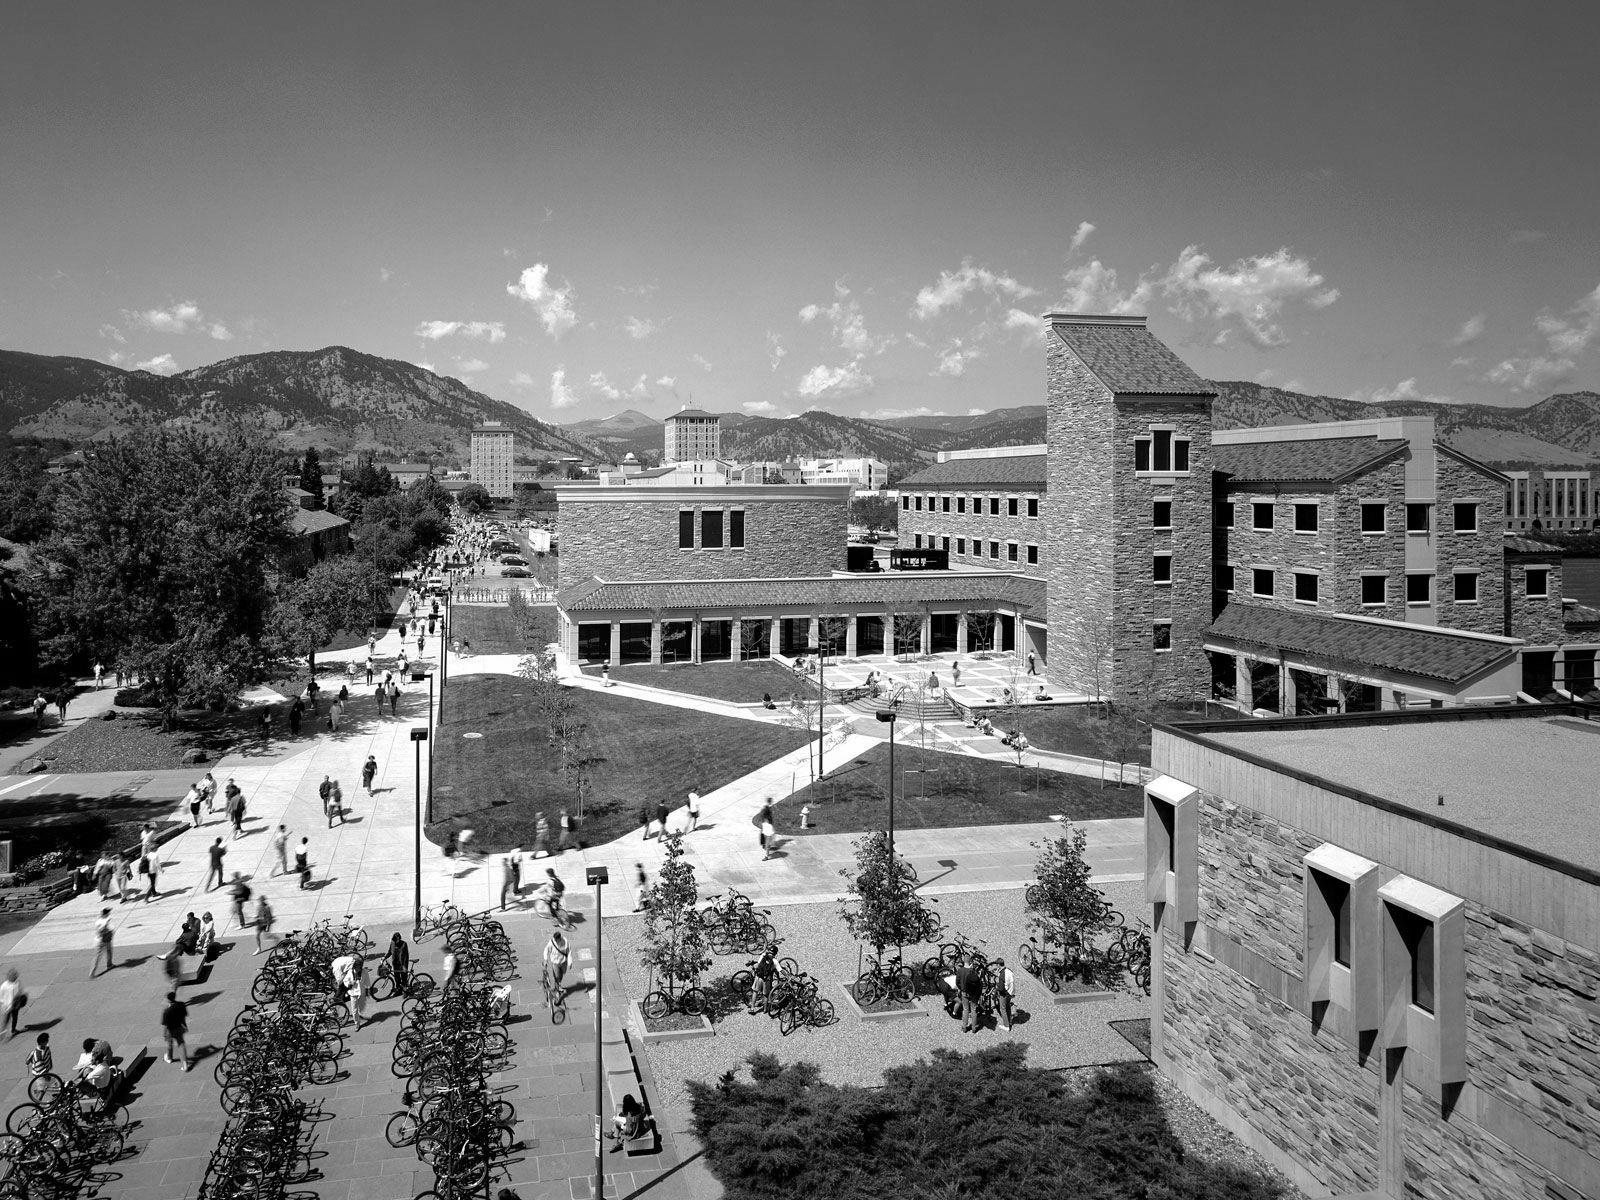
\includegraphics[width=\textwidth]{figs/test01_gray}
		\caption{Before edge detection}
		\label{fig:test01_gray}
	\end{subfigure}
	\par
	\begin{subfigure}[h]{0.7\textwidth}
		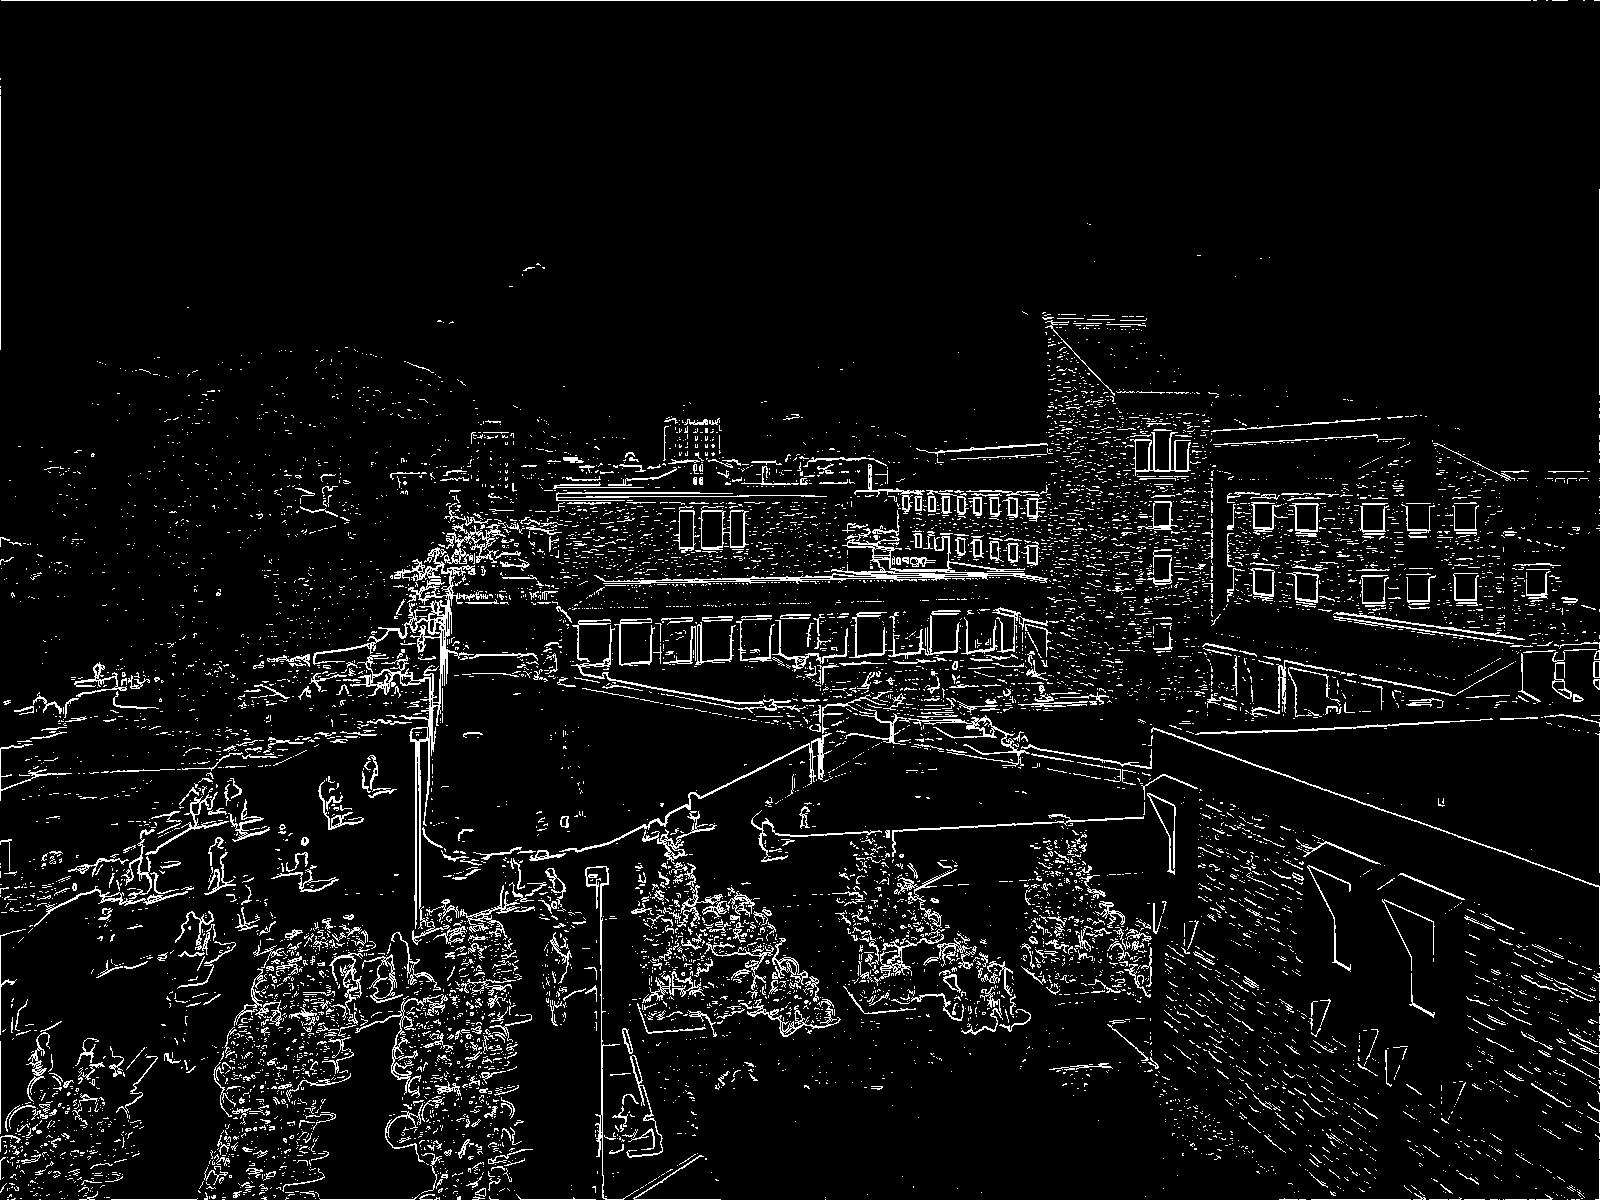
\includegraphics[width=\textwidth]{figs/test01_edges}
		\caption{After edge detection}
		\label{fig:test01_edge}
	\end{subfigure}
	
	\caption{Sobel edge detection with a threshold intensity of 80.}
	\label{fig:edge01}
\end{figure}

This looks pretty good! People walking stand out well from the sidewalk, building features are well defined, grass/sidewalk boundaries are detected. However, the foothills are washed out and there are still some artifacts from clouds and such. It wouldn't work for the fill tool in MS paint, but it's a good start. A threshold of 80 was chosen over 70, because there is reduced noise (artifacts) with a higher threshold. 70 defines the foothills and clouds a little better.

\pagebreak

\begin{figure}[ht]
	\centering
	\begin{subfigure}[h]{0.75\textwidth}
		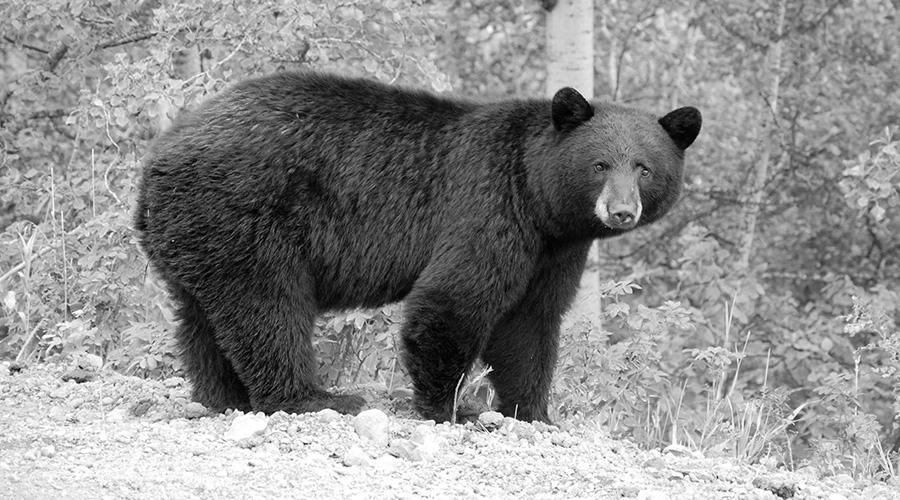
\includegraphics[width=\textwidth]{figs/test02_gray}
		\caption{Before edge detection}
		\label{fig:test02_gray}
	\end{subfigure}
	\par
	\begin{subfigure}[h]{0.75\textwidth}
		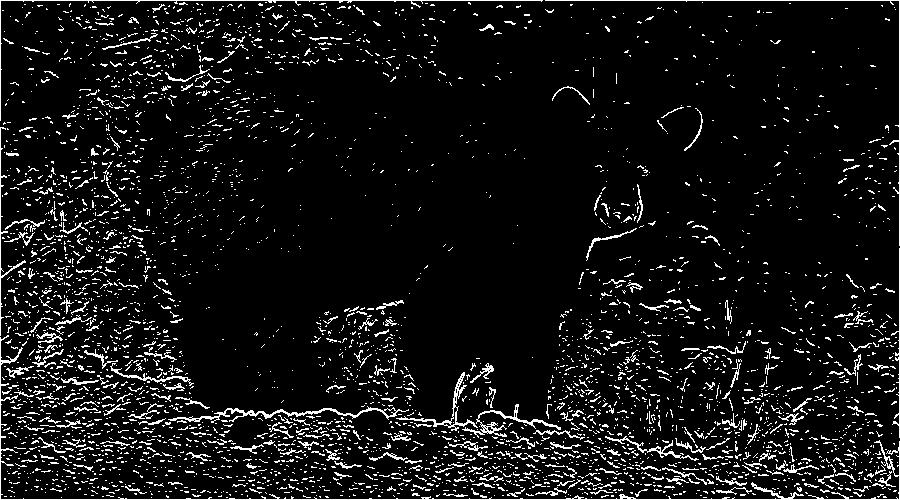
\includegraphics[width=\textwidth]{figs/test02_edges}
		\caption{After edge detection}
		\label{fig:test02_edge}
	\end{subfigure}
	
	\caption{Sobel edge detection with a threshold intensity of 60.}
	\label{fig:edge02}
\end{figure}

In contrast to the image in \ref{fig:edge01}, we have a bear in nature in fig. \ref{fig:edge02}. It is clear that the algorithm does not work as well for this image. The leaves in the background are detected as edges more prominently than the outline of the bear. We do get a relatively clear outline of his ears and other facial features. Here, at least, one could theoretically take the dense white background and subtract it from the sparse outline of the bear if the wish was to extract the bear from the background. Obviously, with a higher threshold, the leaves are not detected as prominently, however with the focus of the image being the bear, I wanted the edges of the ears and face to be well defined and thus chose this image with a threshold of 60.

\textbf{Lab question 7:} I think we may have gotten better results with edge detection of the bear in fig. \ref{fig:edge02} by processing the color image because the background is a somewhat uniform color and contrasts with the bear. Processing the RGB channels separately would be helpful in extracting all features of one color or detecting steep gradients between different objects when their colors are different.

\pagebreak

\section{Image Resizing}

\subsection{Introduction}
Resizing images happens all the time. Whether it is data storage space that one wishes to conserve, or fitting a small image to fit your desktop display background, the image must be resized. How this is accomplished can be done in a few different ways. In this lab, we will only focus on a relatively simple, but still effective, and not terribly low quality method. We will call the process of shrinking an image, "downsampling" and expanfing it, "upsampling". As these names imply, we will have to choose a subset of the pixels to include in an image when shrinking it (or build a new, smaller collection of pixels) and introduce new pixel values to fill in for empty space in the enlarged image.

\paragraph{Downsampling} Rather than simply including every 4th pixel, for example, in a new smaller image, we will use averaging to smooth the effect of scaling down. We consider the scaling factor, $N$, such that an original image with $R$ rows and $C$ columns will produce a new image of size $R/N$ by $C/N$. We accomplish this by dividing the image into blocks of size $N \times N$, averaging the intensity of each block to obtain a new intensity for one pixel in the smaller output image.

\paragraph{Upsampling} Enlarging an image is a little more complicated, as we need to introduce new information. The process of upsampling is generally called interpolation. There are also multiple ways to do this, such as linear, cubic, etc. In addition, we need to interpolate in 2 dimensions, wo we will use bi-linear interpolation. Fortunately, \verb|scipy.interpolate| has a function, \verb|RectBivariateSpline| to help do this.

\begin{figure}[ht]
	\centering
	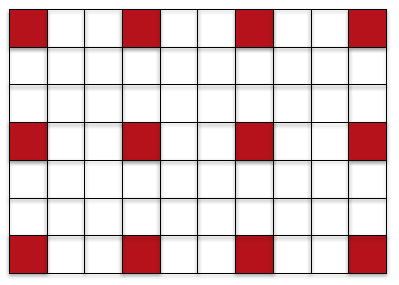
\includegraphics[scale=1]{figs/upsample}
	\caption{Geometrically, we need to space pixels in the original image out by N pixels. Interpolation is necessary to fill in the missing pixel values with meaningful information.}
	\label{fig:upsample_graphic}
\end{figure}

\begin{figure}[ht]
	\centering
	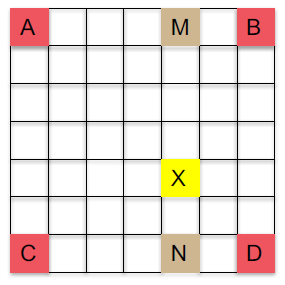
\includegraphics[scale=1.3]{figs/bilinear_interp}
	\caption{Graphical representation of bilinear interpolation.}
	\label{fig:bl_int}
\end{figure}

To find $X$ in fig. \ref{fig:bl_int}, we first need to find $M$ using a linear interpolation between $A$ and $B$. Then we need to find $N$ using linear interpolation between $C$ and $D$. Finally, we can linearly interpolate between $M$ and $N$ to find $X$. 

\pagebreak

\subsection{Method}
We will implement this part of the lab using relatively slow \verb|for()| loops and touch every pixel in the original array.
\paragraph{Downsampling} There are a few ways to do this. I chose to loop over $N \times N$ size blocks of the original image, but one could also loop over each pixel of the new image. For my implementation, I used array splicing in Python to extract a block, and \verb|numpy.average| to obtain a new pixel value. 

\begin{lstlisting}[language=Python]
# declare new, smaller image
imageOut = np.zeros([(int)(np.shape(imageIn)[0] / N), (int)(np.shape(imageIn)[1] / N)])
xIndex = 0
yIndex = 0
# loop over x dim
for blockX in range(0, np.shape(imageIn)[0], N):
    # loop over y dim
    for blockY in range(0, np.shape(imageIn)[1], N):
        sample = imageIn[blockX:blockX + N, blockY:blockY + N]
        imageOut[xIndex,yIndex] = np.average(sample)
        yIndex += 1
    yIndex = 0
    xIndex += 1
\end{lstlisting}

\paragraph{Upsampling}
\verb|RectBivariateSpline| has input arguments of an array of x-indexes, an array of y-indexes, and an array of intensities at the given indexes. So, we begin by looping over all the pixels. Inside this loop, we define each range of $x$ and $y$ values to be the current pixel and its adjacent neighbor in the original pixel array. We define $z$ to be the intensities at those locations. Building an instance of the interpolation object and passing it $x$, $y$, and $z$, we obtain a new array containing the original values with interpolated values between. We assign this array to the output image and continue looping over the image. 

\begin{lstlisting}[language=Python]
# declare new, larger image
imageOut = np.zeros([(int)(np.shape(imageIn)[0] * N), (int)(np.shape(imageIn)[1] * N)])
xIndex = 0
yIndex = 0
# loop over every x pixel in input image
for pixelX in range(np.shape(imageIn)[0] - 1):
    # loop over every y pixel in input image
    for pixelY in range(np.shape(imageIn)[1] - 1):
        # bi-linear interpolation
        # x and y hold indices of pixels used for interpolation
        x = np.asarray([pixelX,pixelX + 1], np.int)
        y = np.asarray([pixelY,pixelY + 1], np.int)
        # z holds intensities at those locations
        z = np.asarray([[imageIn[pixelX,pixelY],imageIn[pixelX,pixelY + 1]],
                        [imageIn[pixelX + 1,pixelY],imageIn[pixelX + 1,pixelY + 1]]], np.float)
        # interpolation object
        interp_spline = sp(y, x, z, kx=1, ky=1)
        # interpolate onto smaller grid
        x1 = np.linspace(pixelX, pixelX + 1, N + 1)
        y1 = np.linspace(pixelY, pixelY + 1, N + 1)
        ivals = interp_spline(y1, x1)
        # spread pixels out and place interpolated values in between
        imageOut[pixelX*N:(pixelX*N) + (N), pixelY*N:(pixelY*N) + (N)] = ivals[0:N,0:N]
\end{lstlisting}

Some of the assignments in the above code excerpt appear fairly complex, but most are really just using the current index + 1 and multiplying by $N$ to index the correct mapping in the larger image array.

\subsection{Results}
First, we took an image and downsampled it by 2. Then, upsampling it by 2 we get the same size image we started with, but with much lower resolution. It's hard to show the difference between the two here, but we can do that in Python. Taking the absolute difference of the original and processed images, we see the result in figure \ref{fig:downup2}.

\pagebreak

\begin{figure}[ht]
	\centering
	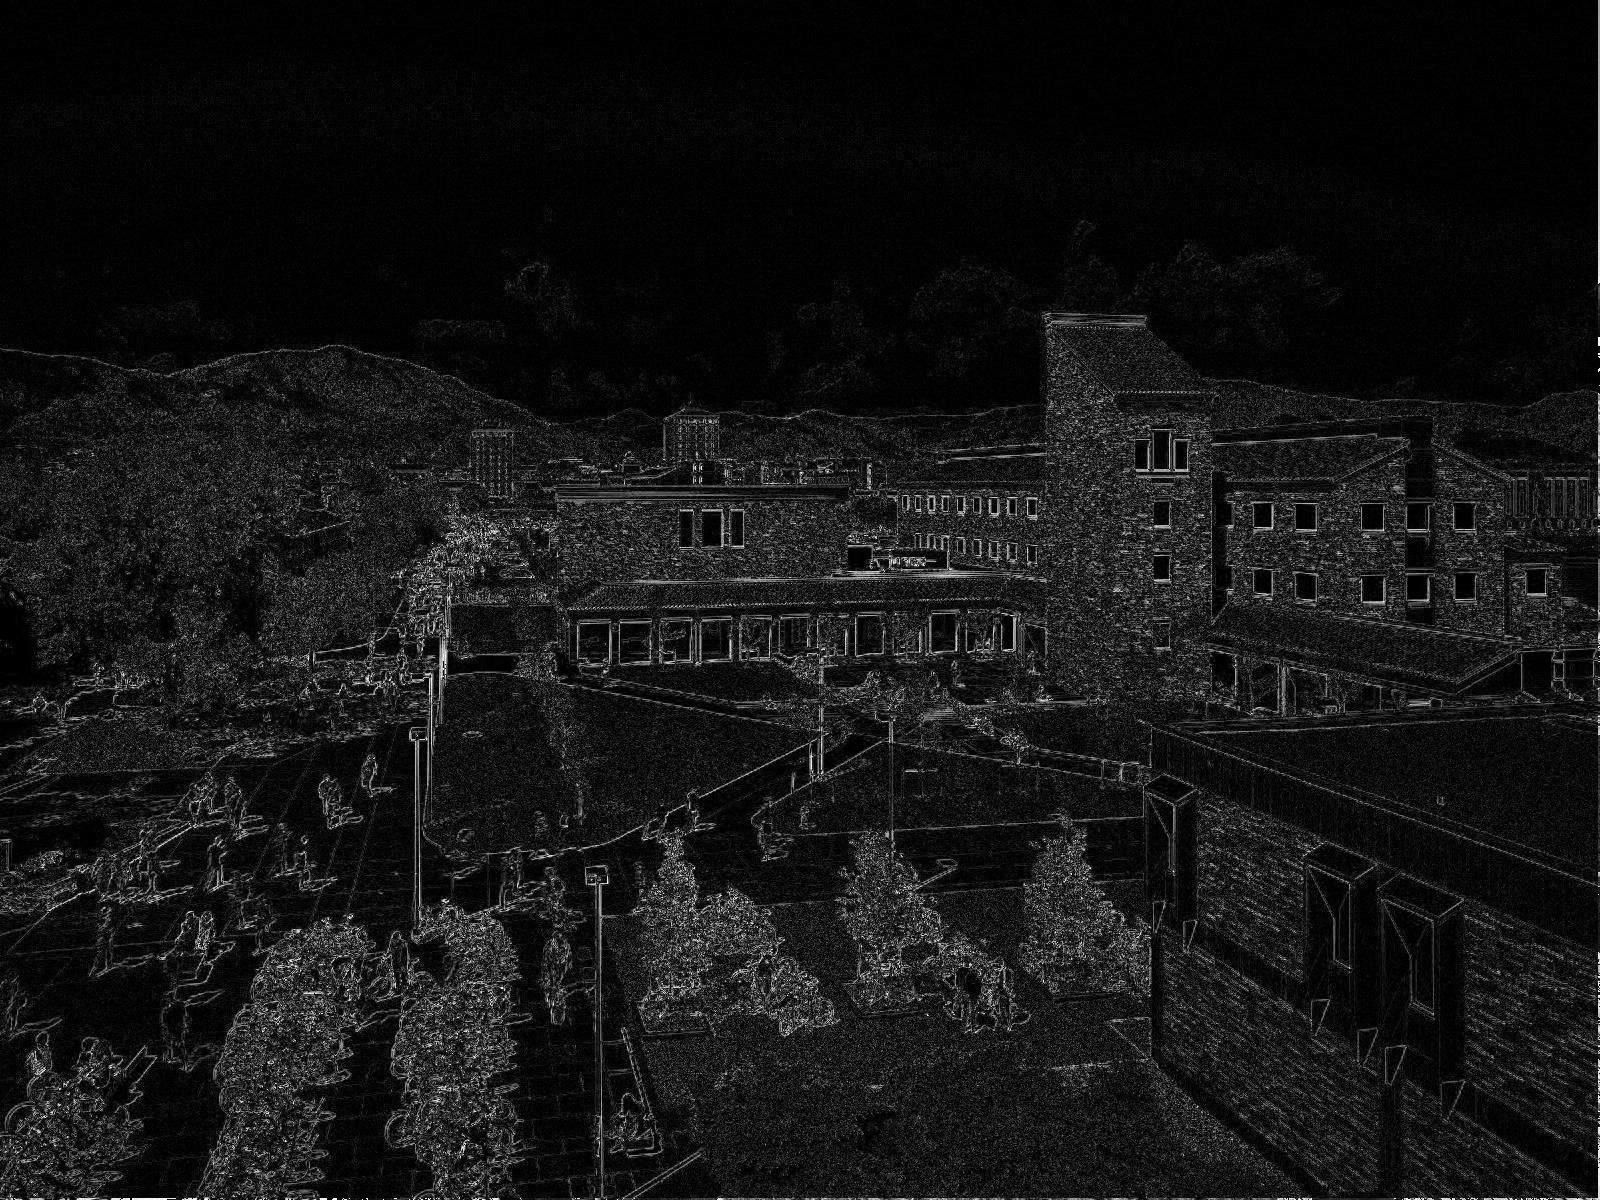
\includegraphics[width=0.9\textwidth]{figs/test01_downUp2_diff2}
	\caption{Absolute difference between an image downsampled by $N=2$, then upsampled by 2.}
	\label{fig:downup2}
\end{figure}

Based on the sharp features in fig. \ref{fig:downup2}, high frequency, or sharp features were lost in the downsampling procedure. This shouldn't be surprising, but it's worse the further we downsample. Shown in figure \ref{fig:downup4} is the same procedure with $N=4$.

\clearpage

\begin{figure}[ht]
	\centering
	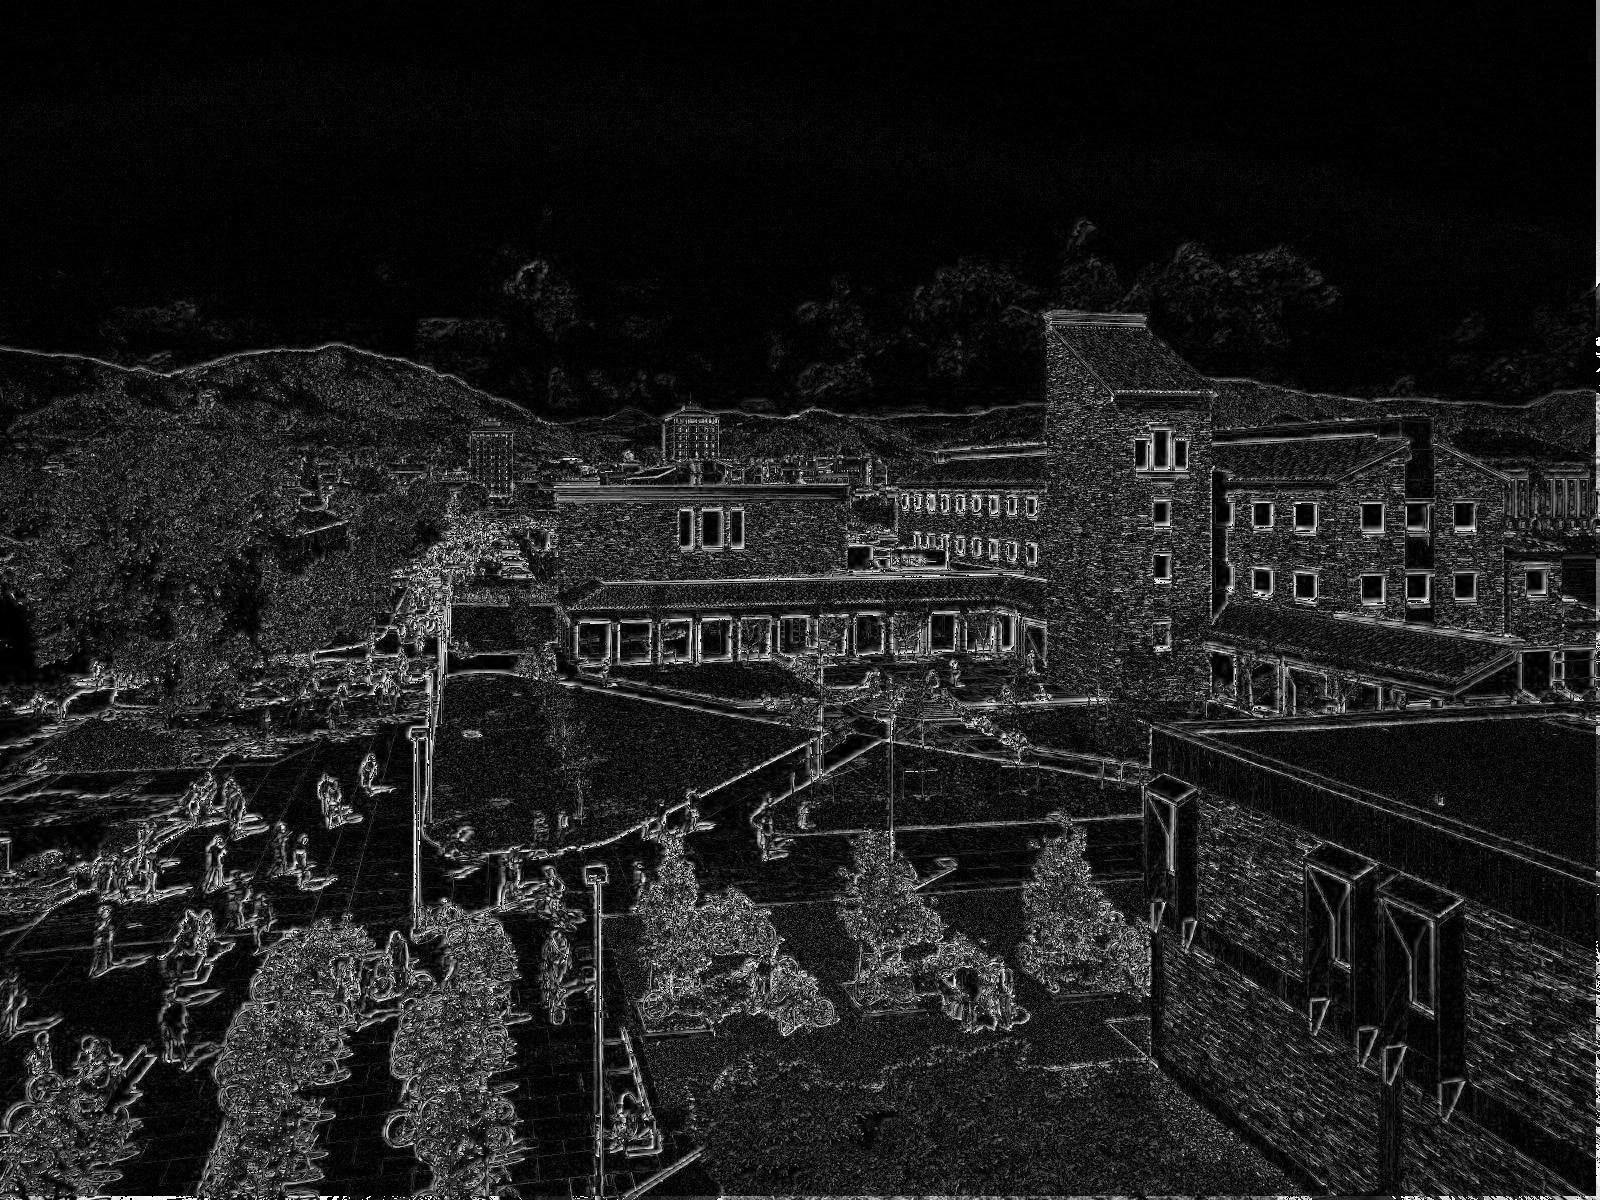
\includegraphics[width=0.9\textwidth]{figs/test01_downUp4_diff2}
	\caption{Absolute difference between an image downsampled by $N=4$, then upsampled by 4.}
	\label{fig:downup4}
\end{figure}

We see again in fig. \ref{fig:downup4} that sharp features were lost, but this time a small region surrounding those features was lost as well. This is due to the linear interpolation method, which creates a blurred region around sharp features, as there is no way to recover the actual information discarded by downsampling.

\clearpage

\section{Conclusion}
This introduction to image processing was exciting. Grayscale conversion is relatively easy and many of these functions could be extended to process color images without much difficulty. One comment is that the nested-loop method for image resizing is terribly inefficient. At least on my computer, the algorithm for upsampling takes minutes to complete, so there's definitely room for optimization. This edge detection algorithm seems fairly rudimentary and I would be very interested in implementing more complex and useful algorithms. I think I am convinced at this point that histogram equalization is not the best way to adjust the contrast of an image. Overall, I am happy with the results of this lab.

\pagebreak

\section{Appendix}
	
\subsection{Appendix A: Grayscale Conversion} \label{app:gray}
	\begin{lstlisting}[language=Python,label={lst:gray}]
def grayscale(image):
    imageIn = np.asarray(image,np.uint8)
    rows = imageIn.shape[0]
    cols = imageIn.shape[1]

    # convert image to grayscale
    Y = [0.299,0.587,0.114]
    imGray = np.dot(imageIn,Y)
    imGray = imGray.astype(np.uint8)

    # convert ndarray into linear array
    linIm = np.reshape(imGray,rows * cols)

    # clip out of bounds values
    linIm = np.where(linIm < 0,0,linIm)
    linIm = np.where(linIm > 255,255,linIm)

    # reshape back into 2D array
    imGray = np.reshape(linIm,[rows,cols])

    return imGray
	\end{lstlisting}
	
\pagebreak
	
\subsection{Appendix B: Histogram Equalization} \label{app:hist}
	\begin{lstlisting}[language=Python,label={lst:hist}]
def histEQ(image):
    image = image.convert('L')
    image = np.asarray(image, np.float)
    hist_before = np.zeros(256, dtype=int)
    # Count frequency of every value in image
    freq = Counter(np.reshape(image, image.shape[0] * image.shape[1]))
    # sort into numpy array
    for p in range(256):
        hist_before[p] = freq[p]
    # declare remapping table and initialize variables
    remap = np.zeros(256, dtype=int)
    remap[-1] = 255
    histSum = sum(hist_before[1:-2])
    P = histSum / 254
    T = P
    outval = 1
    curr_sum = 0
    # build remap table
    for inval in range(1, 255, 1):
        curr_sum += hist_before[inval]
        remap[inval] = outval
        if (curr_sum > T):
            outval = round(curr_sum/P)
            T = outval*P
    # declare output image
    image_equalized = np.zeros_like(image)
    # remap intensities into equalized array
    for intensity in range(256):
        # remap values to equalize
        image_equalized = np.where(image == intensity, 
                                   remap[intensity], 
                                   image_equalized)
    # compute histogram after equalization
    hist_after = np.zeros(256,dtype=int)
    # count value occurrences
    freq = Counter(np.reshape(image_equalized,image_equalized.shape[0] 
                              * image_equalized.shape[1]))
    # sort
    for p in range(256):
        hist_after[p] = freq[p]
    return image_equalized, hist_before, hist_after, remap, image
    \end{lstlisting}
    
\pagebreak
    
\subsection{Appendix C: Edge Detection} \label{app:edge}
    \begin{lstlisting}[language=Python,label={lst:edge}]
def Sobel(imageIn, thresh):
    # convert to grayscale
    imageIn = np.asarray(imageIn.convert('L'), np.float)
    convolved = np.zeros_like(imageIn)
    # Sobel kernels
    df_dy = np.array([[-1, -2, -2],
                     [0, 0, 0],
                     [1, 2, 1]])
    df_dx = np.array([[-1, 0, 1],
                     [-2, 0, 2],
                     [-1, 0, 1]])
    # perform convolution
    convX = signal.fftconvolve(imageIn, df_dx, mode='same')
    convY = signal.fftconvolve(imageIn, df_dy, mode='same')
    # find the magnitude of the gradient for every pixel
    gradient = np.sqrt( (convX**2) + (convY**2) )
    # normalize
    gradient = (gradient/np.amax(gradient)) * 255
    # detect edges based on threshold value
    imageOut = np.where(gradient < thresh, 0, 255)
    return imageOut
	\end{lstlisting}
	
\subsection{Appendix D: Downsampling} \label{app:downsample}
	\begin{lstlisting}[language=Python]
def scaleDown(imageIn, N):
    # convert to grayscale
    imageIn = np.asarray(imageIn.convert('L'), np.float)
    # declare new, smaller image
    imageOut = np.zeros([(int)(np.shape(imageIn)[0] / N), 
                         (int)(np.shape(imageIn)[1] / N)])
    xIndex = 0
    yIndex = 0
    # loop over x dim
    for blockX in range(0, np.shape(imageIn)[0], N):
        # loop over y dim
        for blockY in range(0, np.shape(imageIn)[1], N):
            sample = imageIn[blockX:blockX + N, blockY:blockY + N]
            imageOut[xIndex,yIndex] = np.average(sample)
            yIndex += 1
        yIndex = 0
        xIndex += 1
    return imageOut
    \end{lstlisting}
    
\pagebreak
    
\subsection{Appendix E: Upsampling}
	\begin{lstlisting}[language=Python]
def upScale(imageIn, N):
    # convert to grayscale
    imageIn = np.asarray(imageIn.convert('L'), np.float)
    # declare new, larger image
    imageOut = np.zeros([(int)(np.shape(imageIn)[0] * N), 
                         (int)(np.shape(imageIn)[1] * N)])
    xIndex = 0
    yIndex = 0
    # loop over every x pixel in input image
    for pixelX in range(np.shape(imageIn)[0] - 1):
        # loop over every y pixel in input image
        for pixelY in range(np.shape(imageIn)[1] - 1):
            # bi-linear interpolation
            # x and y hold indices of pixels used for interpolation
            x = np.asarray([pixelX,pixelX + 1], np.int)
            y = np.asarray([pixelY,pixelY + 1], np.int)
            # z holds intensities at those locations
            z = np.asarray([[imageIn[pixelX,pixelY],
                             imageIn[pixelX,pixelY + 1]],
                            [imageIn[pixelX + 1,pixelY],
                             imageIn[pixelX + 1,pixelY + 1]]], np.float)
            # interpolation object
            interp_spline = sp(y, x, z, kx=1, ky=1)
            # interpolate onto smaller grid
            x1 = np.linspace(pixelX, pixelX + 1, N + 1)
            y1 = np.linspace(pixelY, pixelY + 1, N + 1)
            ivals = interp_spline(y1, x1)
            # spread pixels out and place interpolated values in between
            imageOut[pixelX*N:(pixelX*N) + (N), pixelY*N:(pixelY*N) + (N)] = ivals[0:N,0:N]
    return imageOut
    \end{lstlisting}
    
\subsection{Appendix F: Difference}
	\begin{lstlisting}[language=Python]
def difference(im1, im2):
    diff = 2*np.abs(im1 - im2)
    np.where(diff > 255, 255, diff)
    return diff
    \end{lstlisting}
    
\pagebreak
	
\subsection{Appendix G: Main} \label{app:main}
	\begin{lstlisting}[language=Python,label={lst:main}]
# -*- coding: utf-8 -*-
"""
Created on Wed Jan 30 15:05:15 2019

@author: Andrew Teta
"""

import matplotlib.pyplot as plt
import numpy as np
from PIL import Image
import glob
import os
from collections import Counter
import lab2_funcs as lf

# ========== Grayscale Conversion =========== #
im1 = Image.open('images/test01.jpg')
# convert image to grayscale
gray1 = lf.grayscale(im1)
# Output grayscale image to file
Image.fromarray(gray1.astype(np.uint8)).save('figs/test01_gray.jpg')
im2 = Image.open('images/test02.jpg')
# convert image to grayscale
gray2 = lf.grayscale(im2)
# Output grayscale image to file
Image.fromarray(gray2.astype(np.uint8)).save('figs/test02_gray.jpg')

# ========== Histogram Equalization =========== #
# lc1
im = Image.open('images/lc1.jpg')
contrast_enhanced_lc1, orig_hist_lc1, post_hist_lc1, remap1, im_out1 = lf.histEQ(im)
Image.fromarray(im_out1.astype(np.uint8)).save('figs/lc1_gray.jpg')
Image.fromarray(contrast_enhanced_lc1.astype(np.uint8)).save('figs/lc1_ce.jpg')
plt.figure(dpi=170)
plt.plot(orig_hist_lc1)
plt.title('Intensity Histogram')
plt.ylabel('Number of pixels')
plt.xlabel('Intensity')
plt.savefig('figs/lc1_hist_bef')
plt.figure(dpi=170)
plt.plot(post_hist_lc1)
plt.title('Intensity Histogram')
plt.ylabel('Number of pixels')
plt.xlabel('Intensity')
plt.savefig('figs/lc1_hist_aft')
plt.figure(dpi=170)
plt.plot(remap1)
plt.title('Remapping Function')
plt.ylabel('Input')
plt.xlabel('Output')
plt.savefig('figs/lc1_remap')
# lc2
im = Image.open('images/lc2.jpg')
contrast_enhanced_lc2, orig_hist_lc2, post_hist_lc2, remap2, im_out2 = lf.histEQ(im)
Image.fromarray(im_out2.astype(np.uint8)).save('figs/lc2_gray.jpg')
Image.fromarray(contrast_enhanced_lc2.astype(np.uint8)).save('figs/lc2_ce.jpg')
plt.figure(dpi=170)
plt.plot(orig_hist_lc2)
plt.title('Intensity Histogram')
plt.ylabel('Number of pixels')
plt.xlabel('Intensity')
plt.savefig('figs/lc2_hist_bef')
plt.figure(dpi=170)
plt.plot(post_hist_lc2)
plt.title('Intensity Histogram')
plt.ylabel('Number of pixels')
plt.xlabel('Intensity')
plt.savefig('figs/lc2_hist_aft')
plt.figure(dpi=170)
plt.plot(remap2)
plt.title('Remapping Function')
plt.ylabel('Input')
plt.xlabel('Output')
plt.savefig('figs/lc2_remap')

# moon
im = Image.open('images/lc3.jpg')
contrast_enhanced_lc3, orig_hist_lc3, post_hist_lc3, remap3, im_out3 = lf.histEQ(im)
Image.fromarray(im_out3.astype(np.uint8)).save('figs/lc3_gray.jpg')
Image.fromarray(contrast_enhanced_lc3.astype(np.uint8)).save('figs/lc3_ce.jpg')

# succulents
im = Image.open('images/succs.jpg')
ce_succs, or_succs, po_succs, rm_succs, out_succs = lf.histEQ(im)
Image.fromarray(out_succs.astype(np.uint8)).save('figs/succs_gray.jpg')
Image.fromarray(ce_succs.astype(np.uint8)).save('figs/succs_ce.jpg')

# ========== Sobel Edge Detection =========== #
# CU
im = Image.open('images/test01.jpg')
for n in range(10, 250, 10):
    edges1 = lf.Sobel(im, n)
    Image.fromarray(edges1.astype(np.uint8)).save('figs/test01_edges' + str(n) + '.jpg')

# bear
im = Image.open('images/test02.jpg')
for n in range(10, 250, 10):
    edges2 = lf.Sobel(im, n)
    Image.fromarray(edges2.astype(np.uint8)).save('figs/test02_edges' + str(n) + '.jpg')

# ========== Scale down by 2, then up by 2 and take the difference =========== #
im = Image.open('images/test01.jpg')
smallImage = lf.scaleDown(im, 2)
Image.fromarray(smallImage.astype(np.uint8)).save('figs/test01_down2.jpg')
downUp = lf.upScale(Image.open('figs/test01_down2.jpg'), 2)
Image.fromarray(downUp.astype(np.uint8)).save('figs/test01_down2_up2.jpg')
diff1 = lf.difference(lf.grayscale(im), downUp)
Image.fromarray(diff1).show()
Image.fromarray(diff1.astype(np.uint8)).save('figs/test01_downUp2_diff2.jpg')

# ========== Scale down by 4, then up by 4 and take the difference =========== #
im = Image.open('images/test01.jpg')
smallImage1 = lf.scaleDown(im, 4)
Image.fromarray(smallImage1.astype(np.uint8)).save('figs/test01_down4.jpg')
downUp1 = lf.upScale(Image.open('figs/test01_down4.jpg'), 4)
Image.fromarray(downUp1.astype(np.uint8)).save('figs/test01_down4_up4.jpg')
diff2 = lf.difference(lf.grayscale(im), downUp1)
Image.fromarray(diff2).show()
Image.fromarray(diff2.astype(np.uint8)).save('figs/test01_downUp4_diff2.jpg')

print ('done')
	\end{lstlisting}

\end{document}